\chapter{Selection of the \BdKstee candidates}
\chaptermark{Chapter5}
\label{Chapter4}
In this chapter the procedure to select \BdKstee candidates is described. This builds the basis for the angular analysis.\\
First the previous \BdKstee analysis is presented and the differences to this analysis are outlined. Then the selection process for the \BdKstee candidates is explained beginning with the preselection and the training of a Boosted Decision Tree to the optimisation of the selection cuts.\\

\section{Previous and current \BdKstee analysis}
Previously a branching ratio measurement of the rare \BdKstee decay in the dilepton mass region from $30\mevcc$ to $1 \gevcc$ has been performed at \lhcb. This analysis was executed on $1 \invfb$ of data collected in 2011 at a center of mass energy of $7 \tev$. 
While the 2011 \lhcb data contained the largest sample of \BdKstee events ever collected this quantity was not enough to perform an angular analysis.  The selected \BdKstee candidates can be seen in Figure \ref{fig:oldsig}.
Before this analysis the only experiments to observe the \BdKstee decay to date are \babar \cite{babar} and \belle \cite{belle}. Each have collected about 30 \BdKstll events in the region of $q^2 < 2\gevcc$ summing over electron and muon final states.\\
\\
The branching ratio measurement of \BdKstee at \lhcb was executed using the \BdToJPsieeKst decay as a normalisation channel and the results were published in the Journal of High Energy Physics \cite{paper}. The measured branching ratio is
\begin{equation}
\BR(\BdKstee)^{30 -1000\mevcc} = (3.1^{+0.9 \ +0.2}_{-0.8 \ -0.3} \pm 0.2) \, 10^{-7}
\end{equation}
where the first uncertainty is statistical, the second systematic, and the third comes from the uncertainties on the branching ratio of the normalisation channel \BdToJPsieeKst. The selected \BdKstee candidates from this analysis can be seen in Figure \ref{fig:oldsig}. As expected, this measurement is in agreement with SM predictions of 
\begin{equation}
\BR(\BdKstee)^{30 -1000\mevcc}_{pred} = 2.43^{+0.66}_{-0.47}\, 10^{-7} \quad \cite{jaeger}.
\end{equation}

\begin{figure}[ht]
\begin{center}
\subfigure{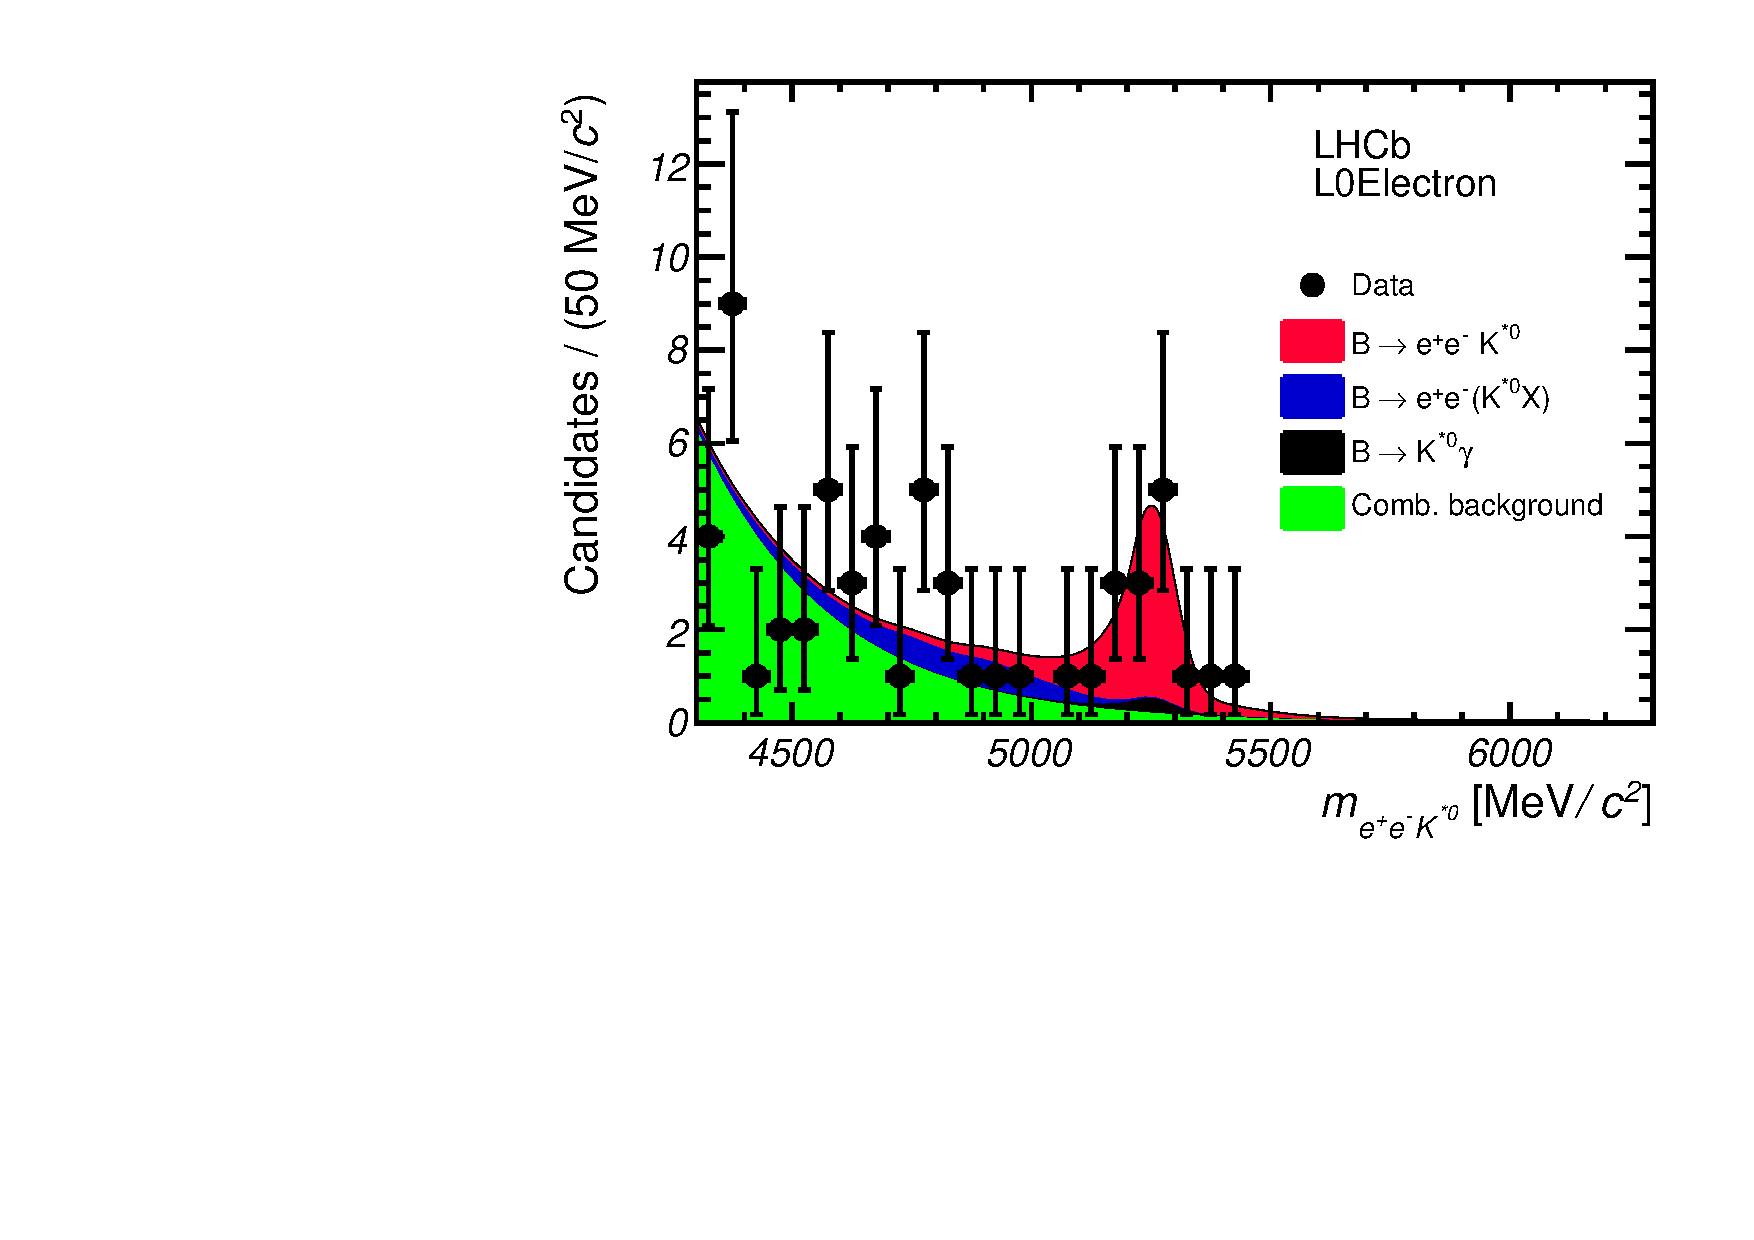
\includegraphics[width = 0.49\textwidth]{L0Ele.pdf}}
\subfigure{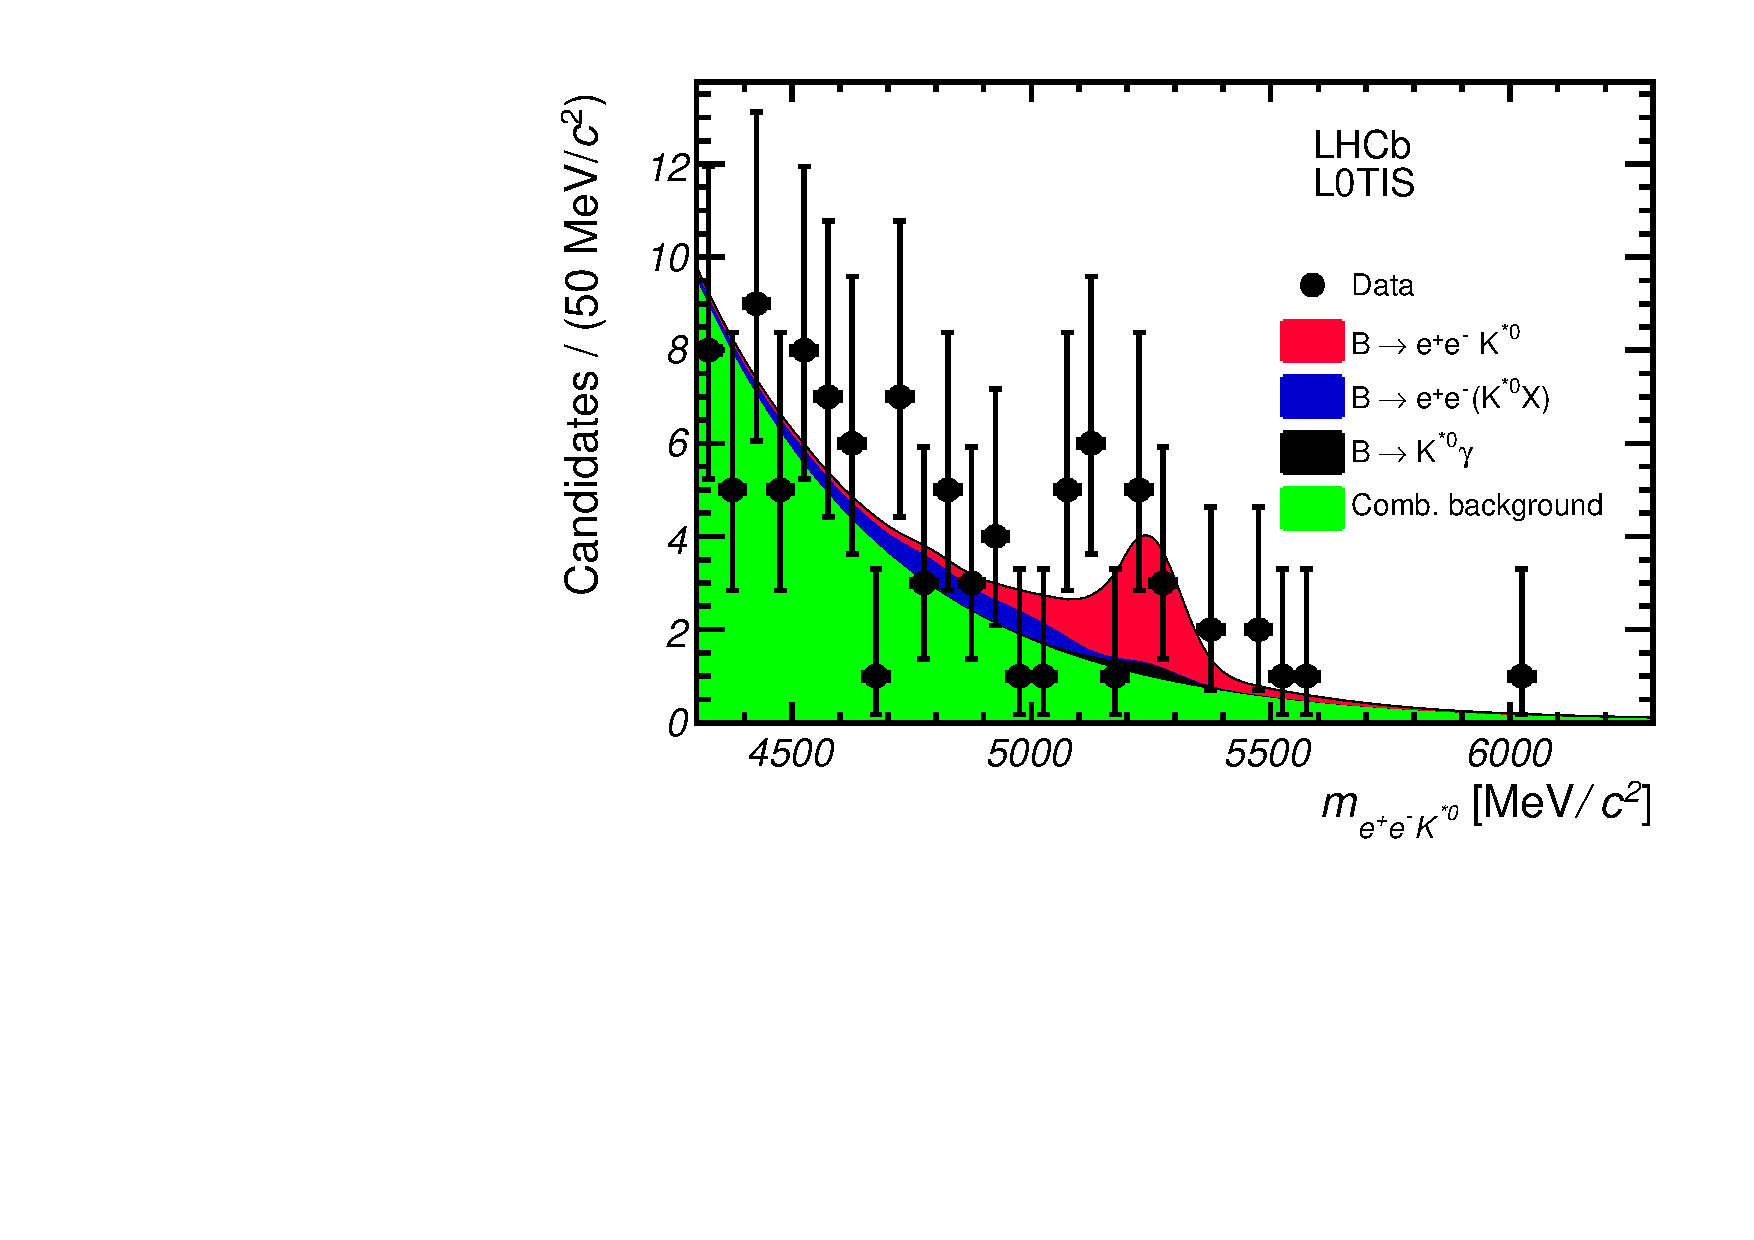
\includegraphics[width = 0.49\textwidth]{L0TIS.pdf}}
\end{center}
\caption{\textit{The \BdKstee candidates obtained from the analysis performed on 1\invfb of \lhcb data collected in 2011 for the two independent trigger categories (see Section \ref{sec:triggercat}).}\cite{paper}}
\label{fig:oldsig}
\end{figure}
While the previous analysis yielded very good results the developed selection was not optimised for 
%selecting \BdKstee candidates for 
an angular analysis on the 2011 and 2012 dataset. The reasons are differing requirements for an angular analysis and several changes in the data-collecting and reconstruction process which will be explored in the following.

\subsection{Selection requirements for an angular analysis}
\label{sec:req}
The selection requirements for an angular analysis are different than those for a branching ratio measurement. 
For the angular analysis it is especially important to have good control over the angular acceptances for the three angles $\theta_l$, $\theta_K$ and $\Phi$ by designing a selection that is as unbiased as possible for these three parameters. Furthermore, the branching ratio measurement was made with respect to the \BdToJPsieeKst as normalisation channel. In that analysis it was important to keep systematic effects between the \BdKstee and the \BdToJPsieeKst channel at a minimum which lead do a different prioritising of the trigger lines.  \\


\subsubsection{Biasing the \ctl acceptance: the $\Bd \rightarrow \Dm \ep \neu$ veto cut}
\label{sec:denu}
The previous analysis used a cut to remove the specific background from the $\Bd \rightarrow \Dm \ep \neu$ decay with the \Dm decaying into \en \Kstarz and \neu. For the $\Bd \rightarrow \Dm \ep \neu $ to pass the \BdKstee selection the neutrinos have to be of very low momentum so that the \Kstarz and the \en share almost the total \Dm energy. To remove the $\Bd \rightarrow \Dm \ep \neu $ background, the invariant mass $m(\Kstarz e)$ of the \Kstarz (\Kstarzb) and the \en (\ep) is calculated and a cut of $m(\Kstarz e) > 1900 \mevcc $ is applied \footnote{$m(\Dm) = 1869 \mevcc$\cite{pdg}}.\\
Unfortunately this cuts biases the \ctl distribution as can be seen in Figure \ref{fig:ctl}. The low momentum neutrinos demand the \Kstarz and the \en to be almost back to back in the rest frame of the \Dm, just as the \Dm and the \ep in the rest frame of the \Bd. This gives the \ep a relatively large energy of $\sim 2 \gev$. For the dielectron invariant mass to be still smaller than $1 \gev$ the \en must be in the opposite direction of the \ep. Therefore the cut against the $\Bd \rightarrow \Dm \ep \neu$ background removes events where \ctl is at high values as illustrated in Figure \ref{fig:ctl}.\\
It is still very important to remove the $\Bd \rightarrow \Dm \ep \neu$ background since the branching ratio for this decay is about four orders of magnitude greater than the branching ratio of the signal decay. To obtain better control over the way the $\Bd \rightarrow \Dm \ep \neu$ veto cut impacts the \ctl distribution the cut on the $m(\Kstarz e)$ is removed and a direct cut $\ctl \, < \, 0.8$ is applied. As can be seen in Figure \ref{fig:kstaremass} the cut on \ctl has almost the same effect on the $m(\Kstarz e)$ distribution as the direct $m(\Kstarz e)$ cut.
\begin{figure}[!h]
\begin{center}
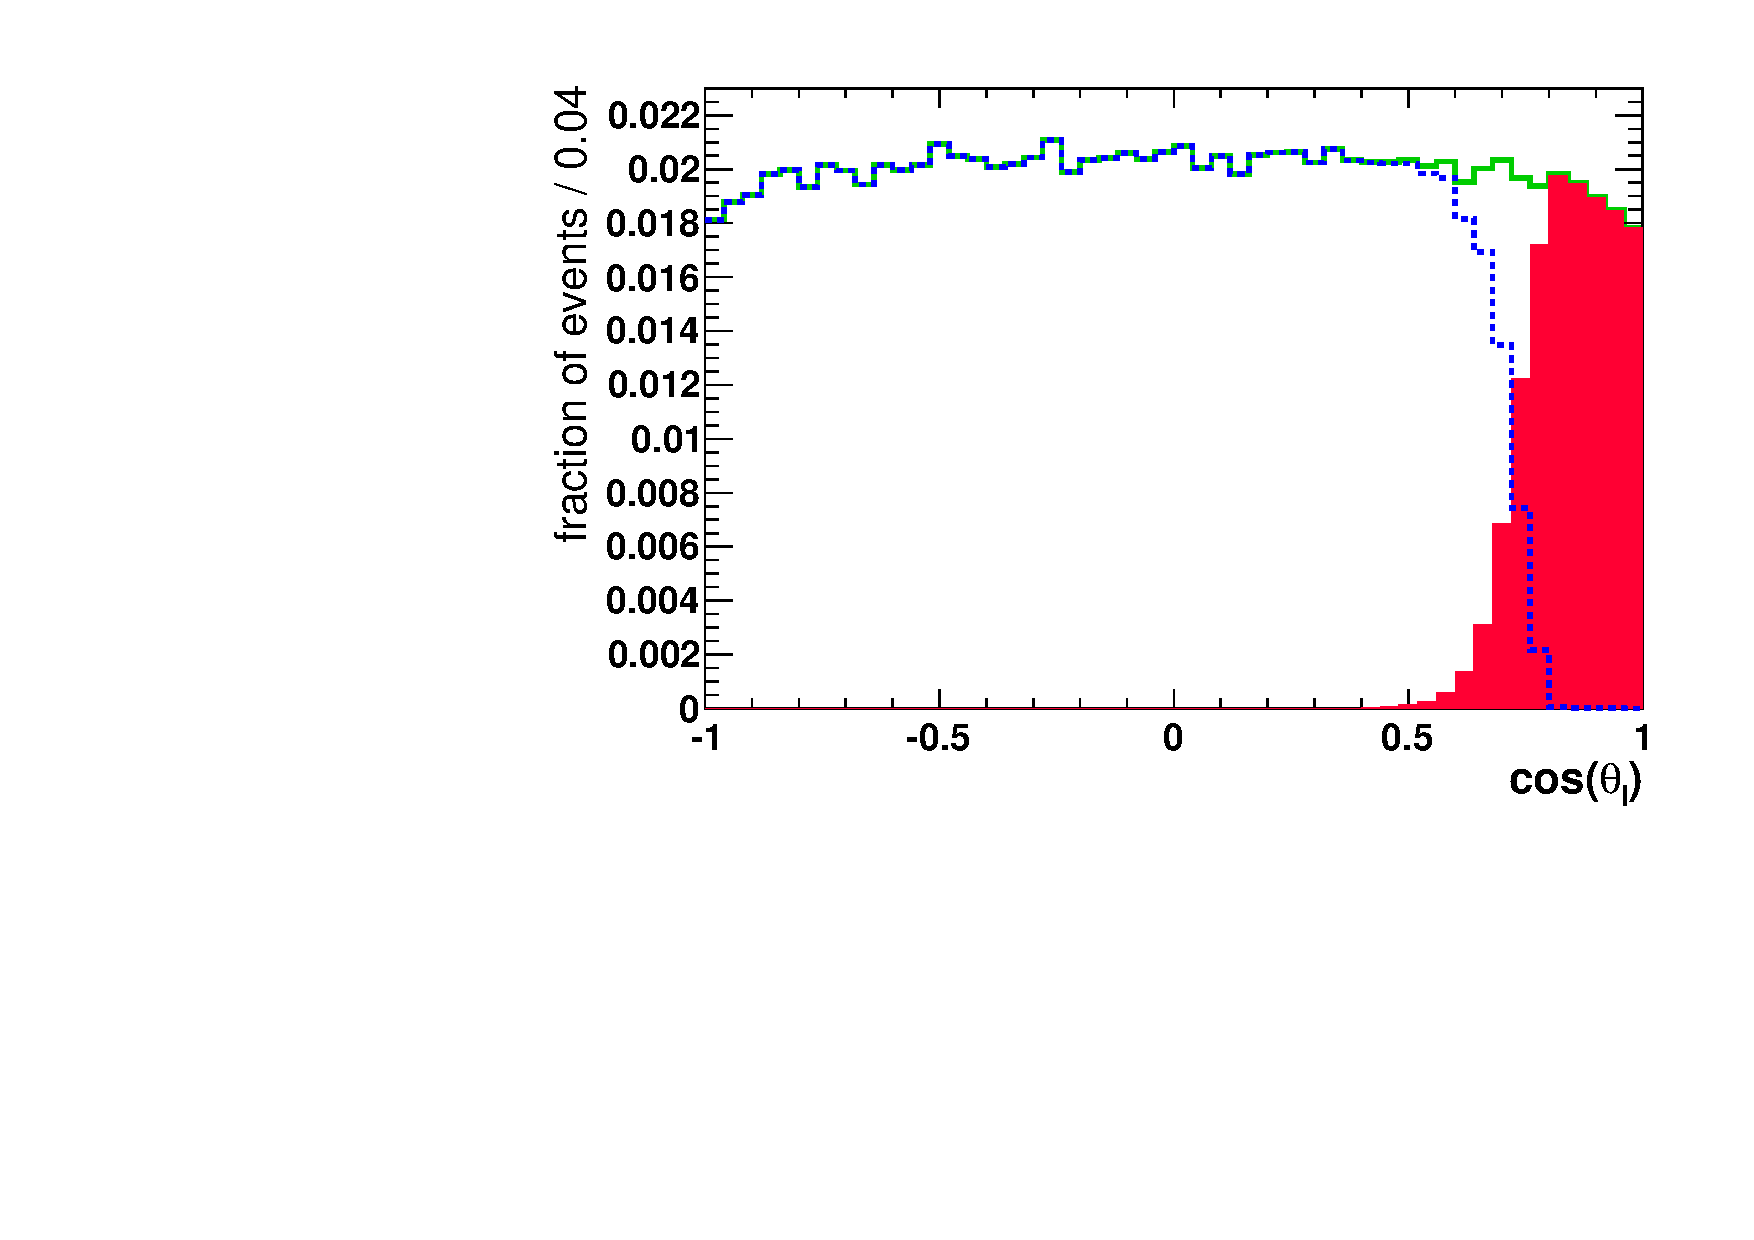
\includegraphics[width = 0.5 \textwidth]{ctl.pdf}
\end{center}
\vspace*{-0.5cm}
\caption{\textit{Illustration of the impact of the $m(\Kstarz e)$ cut on the acceptance of \ctl. Distributions obtained from \BdKstee Monte Carlo that was generated flat in \ctl. Green distribution: \ctl distribution after the stripping, blue dashed distribution: \ctl distribution after the stripping and the  $m(\Kstarz e) > 1900 \mevcc $ cut, pink distribution: events that are removed by the $m(\Kstarz e)$ cut.}}
\label{fig:ctl}
\end{figure}

\begin{figure}[!h]
\begin{center}
\subfigure{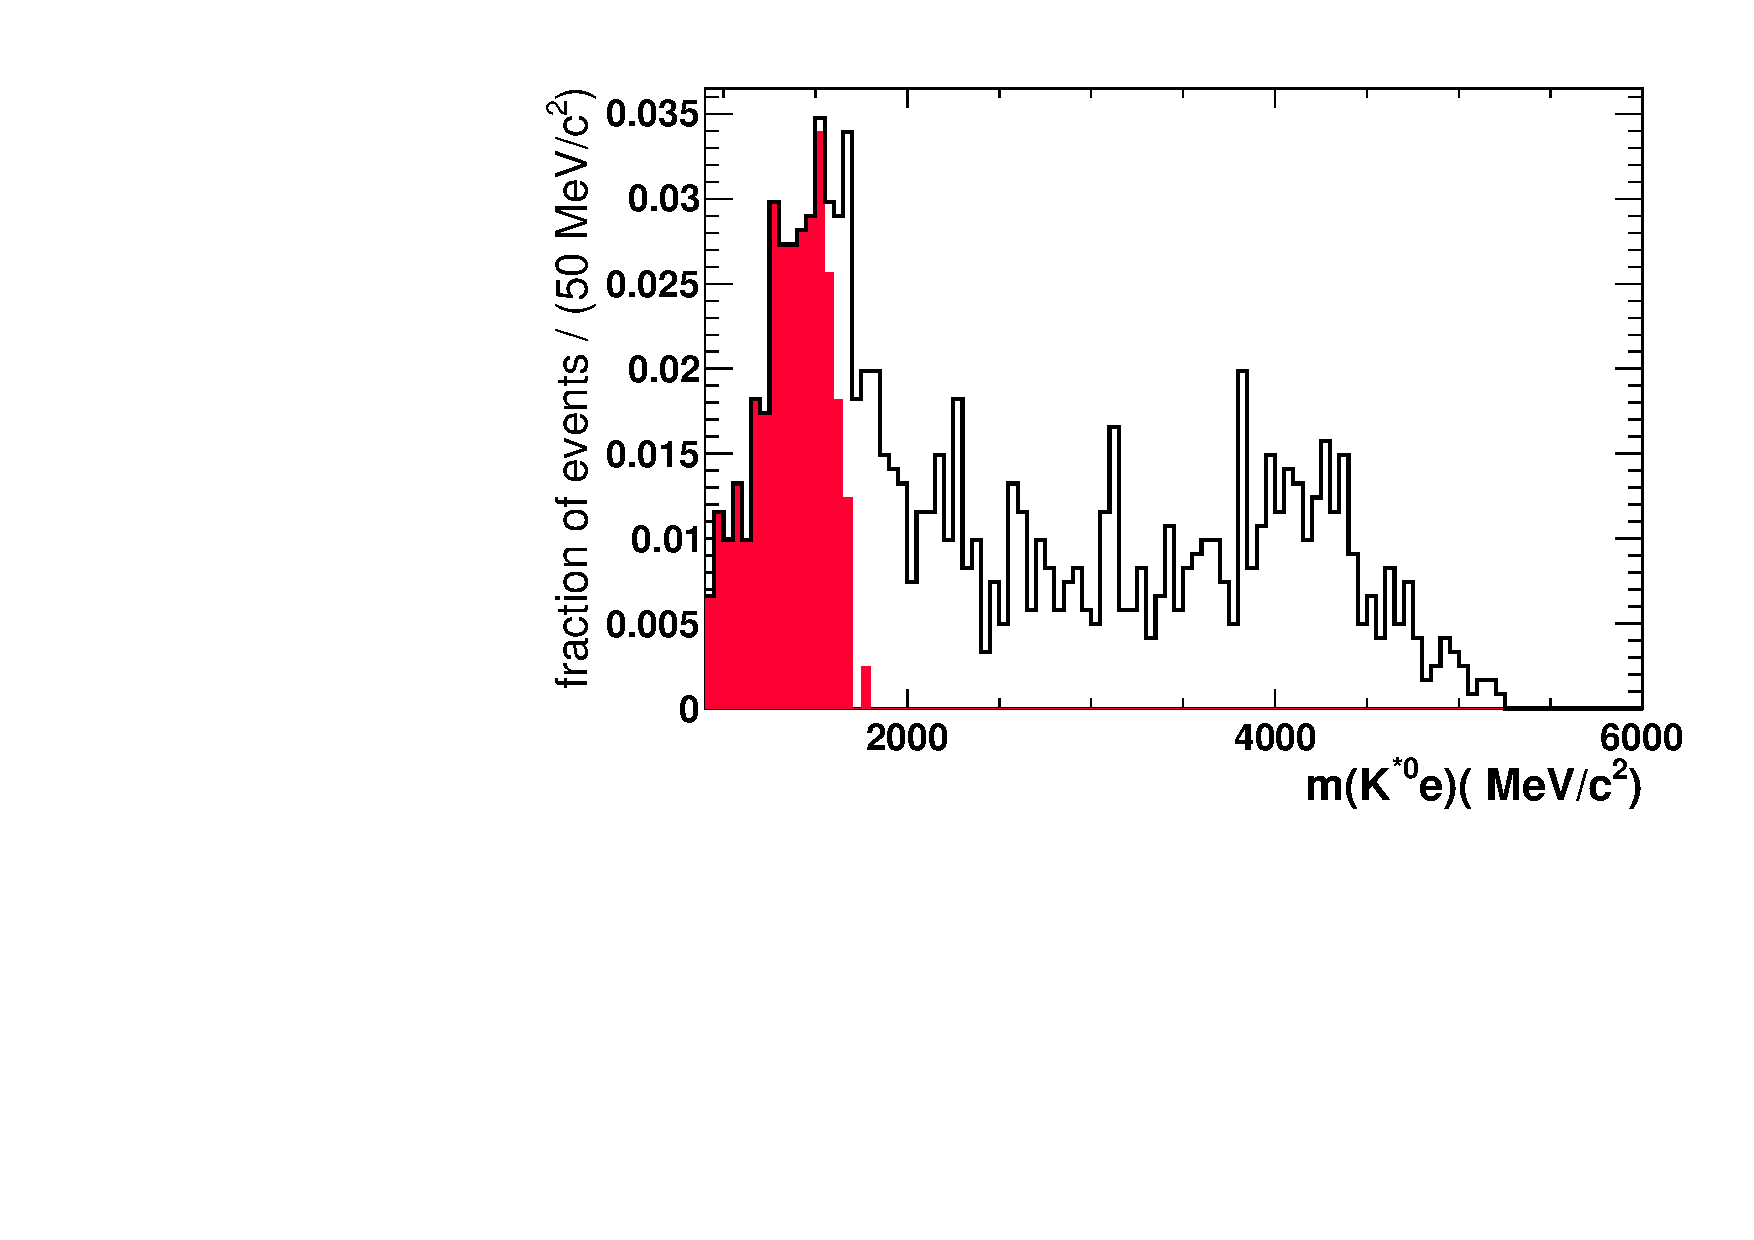
\includegraphics[width=0.49\textwidth]{kstaremass.pdf}}
    \subfigure{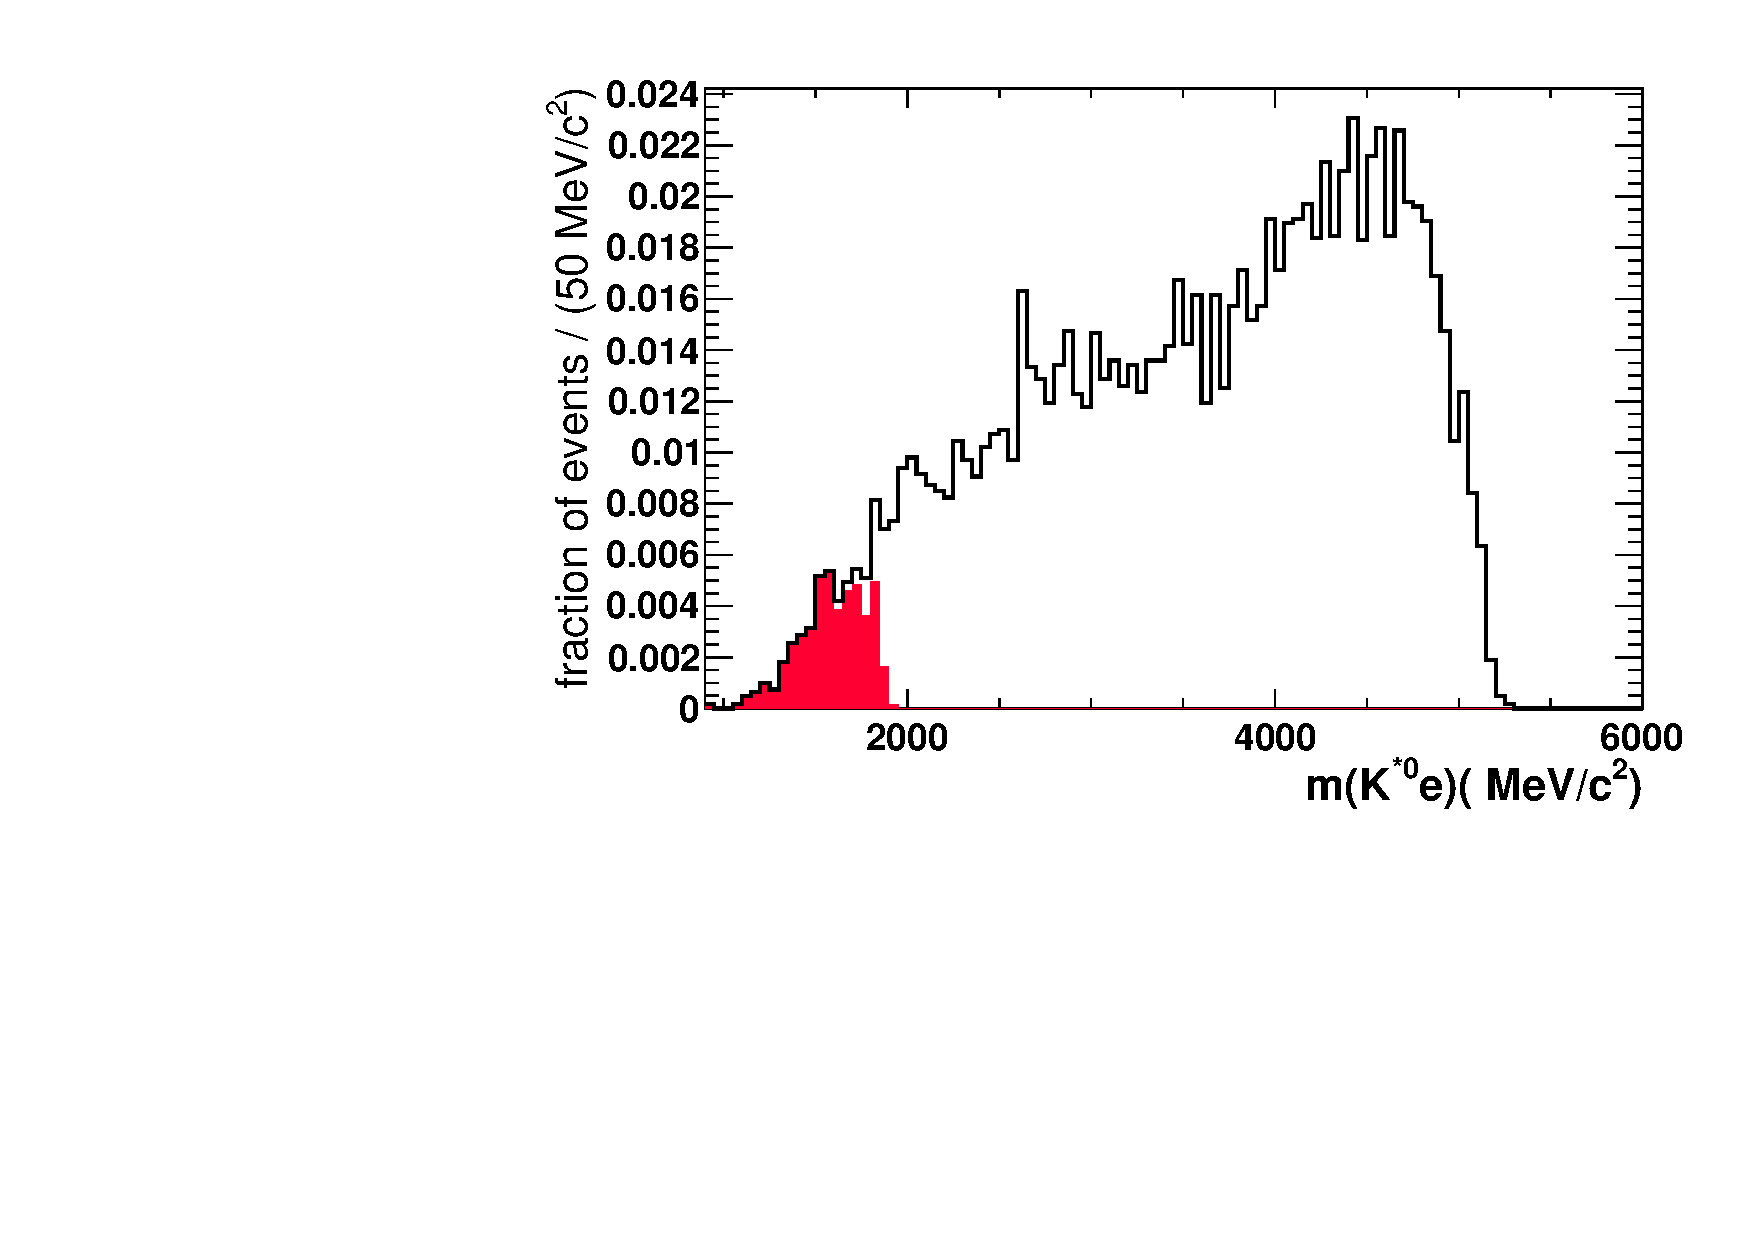
\includegraphics[width=0.49\textwidth]{mckstaremass.pdf}}
\end{center}
\vspace*{-0.8cm}
\caption{\textit{The distribution of the $m(\Kstarz e)$ variable for the \BdKstee candidates after the stripping. Right: \lhcb data from 2011 and 2012, left: \BdKstee Monte Carlo. Pink distribution: candidates that will be removed by the $\ctl \, < \, 0.8$.}}
\label{fig:kstaremass}
\end{figure}
\\
\subsubsection{The mutually exclusive trigger categories}
\label{sec:triggercat}
Due to the different systematics for events in different trigger categories the \BdKstee analysis was and will be performed separately for different independent trigger categories. For the 2011 analysis this categories were the \textit{L0TIS} and the \textit{L0Electron without L0TIS}.\\
The \textit{L0TIS} (L0 Trigger Independent of Signal) candidates are the events where the L0 is triggered by a track that does not come from the signal tracks but from any other track in the detector. The candidates in any \textit{L0TOS} (L0 Trigger On Signal) category are the events where one of the tracks from the \BdKstee candidate enabled the L0 trigger. The candidates that are \textit{L0ElectronTOS} are those that enabled the L0Electron trigger.\\
Obviously some candidates can be L0TIS and L0TOS at the same time, therefore a hierarchy between the trigger categories has to be defined.
The 2011 order was chosen because the \textit{L0TIS} category is obviously independent of the signal decay while the \textit{L0ElectronTOS without L0TIS} induces some systematic differences due to the different momentum distributions of the electrons from \BdKstee and \BdToJPsieeKst. \\
For the angular analysis, the trigger categories were chosen to the:
\begin{itemize}
\item \textbf{L0ElectronTOS}: signal candidate has triggered the L0Electron line
\item \textbf{L0HadronTOS} without L0ElectronTOS: signal candidate has triggered the L0Hadron line but not the L0Electron line
\item \textbf{L0TIS} without L0ElectronTOS and L0HadronTOS: any L0 line was triggered by a track in the event that did not belong to the signal candidate
\end{itemize}
This order was chosen because the events that were triggered by one of the signal candidates (the TOS events) have a cleaner signature as can be seen in Section \ref{sec:fitstrat}.\\
No kind of \textit{L0Hadron} category was used in the 2011 selection because no significant signal could be obtained on the dataset in this category.\\


\subsection{The trigger configurations}
Due to the increase in center of mass energy from $7\tev$ in 2011 to $8\tev$ in 2012, the L0 trigger settings had to be adapted to cope with the increase in the rate of visible interactions and their thresholds were changed several times in 2012. The \BdKstee analysis is most affected by the change in the L0Electron line because of the very low $p_T$ electrons. The threshold energies for the L0Electron trigger line in 2011 and 2012 are listed in Table \ref{tab:loele}. 
\begin{table}[ht]
\begin{center}
\begin{tabular}{c|c|c}
Year & $E_T > $ [\mev] & Recorded luminosity [\invfb]\\
\hline
\hline
2011 & 2500 & 1 \\
\hline 
2012 & 2500 & 0.066 \\
& 2720 & 1.166 \\
& 2860 & 0.260\\
& 2960 & 0.571 \\
\end{tabular}
\caption{\textit{Threshold energies for the L0Electron Trigger in 2011 and 2012.}}
\label{tab:loele}
\vspace*{-0.5cm}
\end{center}
\end{table}

The L0Electron trigger efficiencies depending on the electron transverse energy for the three highest threshold energies are shown in Figure \ref{fig:trigger}. The trigger efficiency is calculated on \BdToJPsieeKst \lhcb data using the \textit{TisTos} method (TIS: Trigger Independant of Signal, TOS: Trigger On Signal) \cite{lopez}. The \BdToJPsieeKst candidates undergo a standard selection and one of the electrons (tag track) must pass a strict selection. The L0Electron efficiency is then calculated using the other electron (probe track). The trigger efficiency depending on the transverse energy of the probe track $E_T$ is calculated by:
\begin{equation}
\epsilon_{L0Ele}(E_T) = \frac{N_{TOS \& TIS}(E_T)}{N_{TIS}(E_T)}
\end{equation}
where $N_{TOS \& TIS}$ denotes the amount of events that are both L0TIS and the probe track triggered the L0Electron and $N_{TIS}$ denotes the events that are L0TIS.

\begin{figure}[ht]
\begin{center}
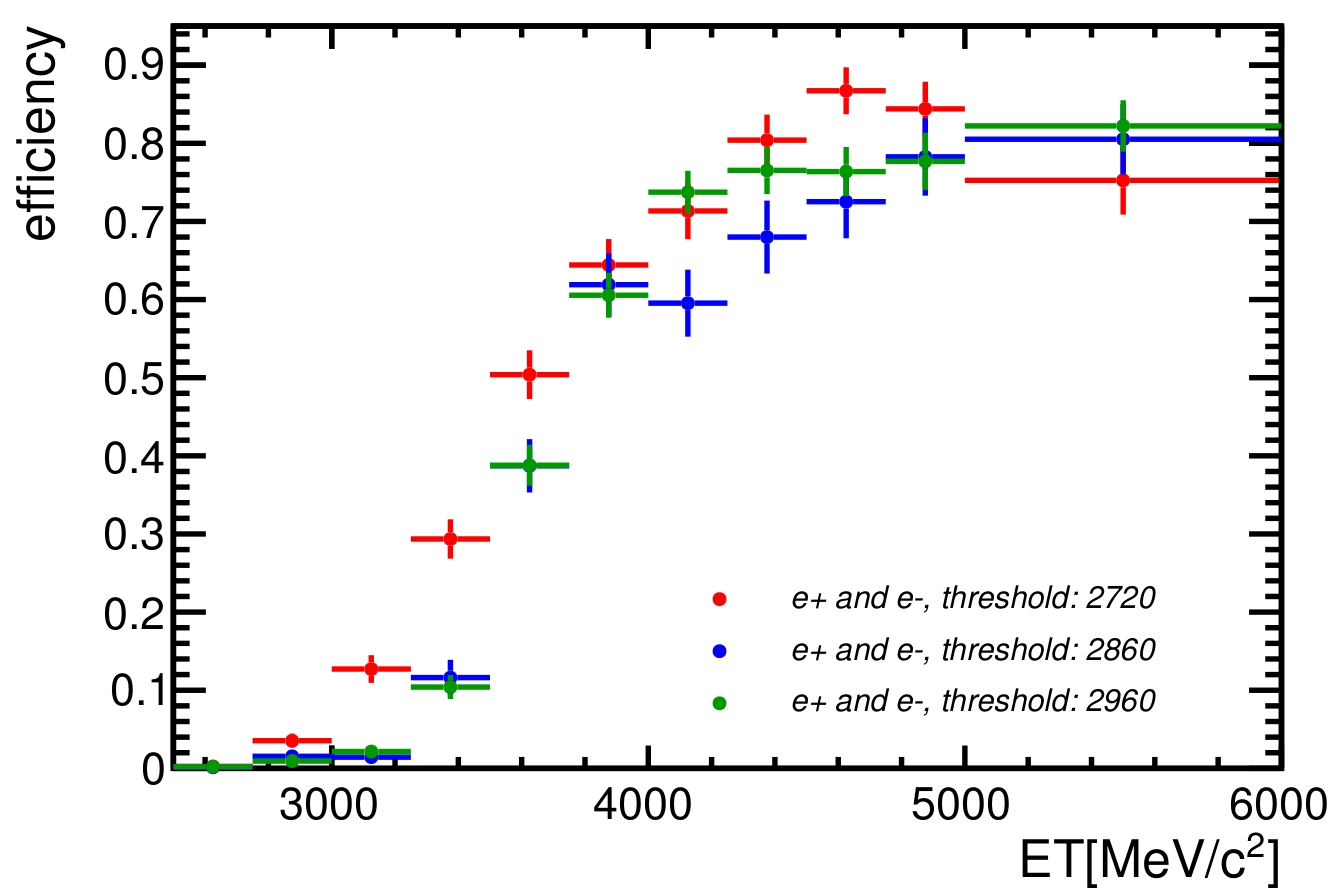
\includegraphics[width = 0.7 \textwidth]{triggereff.jpg}
\end{center}
\vspace*{-0.5cm}
\caption{\textit{The L0Electron efficiency depending on the electron transverse energy for the three different trigger settings.}}
\label{fig:trigger}
\end{figure}
Note that the curves in Figure \ref{fig:trigger} gradually increase around the threshold energy instead of showing a sharp step. This is due to the fact that the energy that triggers the L0Electron is not exactly equal to the reconstructed electron energy. In the reconstruction the electron energy is determined by examining clusters of $3\times 3$ cells in the \ecal while the readout for the L0Electron is performed on clusters of $2\times 2$ cells.\\
The threshold for the L0Hadron trigger was stable at 3.5\gevcc.\\

\subsection{The \BdKstee stripping line}
\label{sec:strips}
A new \BdKstee stripping line was developed after the 2011 analysis. While the 2011 stripping line (\textit{Stripping17b}) was purely cut-based, the new stripping line (\textit{Stripping20}) contains a Boosted Decision Tree (see Section \ref{sec:bdt}) selection and implements the newly developed DiElectronMaker that was introduced in Chapter \ref{chapter3}. After the processing of the 2012 \lhcb data with the \textit{Stripping20} the entire 2011 dataset was reprocessed with \textit{Stripping20} also.\\
\\
The \textit{Stripping20} \bdtn was trained on \BdKstee Monte Carlo as signal sample and background sample was taken from a 2011 \lhcb sample containing mostly hadronic decays. The input variables for the \bdtn are listed in Table \ref{tab:stripbdt} and are very similar to those used in the previous cut-based stripping (for details on \textit{Stripping17b} see Appendix \ref{ap:strip17}), namely the transverse momentum $p_T$ of all seven particles, the impact parameter significance $\chi^2_{(IP)}$ of all seven particles, the flight distance significance $\chi^2_{(FD)}$ of the \Bd, the \Kstarz and the intermediate (\epem) and the angle between the direction of the \Bd candidate momentum and the direction between the primary vertex and the \B decay vertex $\theta_{flight}$. The list of the variables used in the \textit{Stripping20} \bdtn are listed in Table \ref{tab:stripbdt}. \newpage

 \renewcommand{\arraystretch}{1.5} 
\begin{table}[ht]
\begin{center}
\begin{tabular}{c|l}
Particle & Variable \\
\hline
\hline
 \Bd & $p_T(\Bd)$,\qquad $\chi^2_{IP}(\Bd)$,\qquad \ \ $\chi^2_{FD}(\Bd)$,\qquad $\theta_{flight}$ \\
\hline 
\Kstarz & $p_T(\Kstarz)$,\qquad $\chi^2_{IP}(\Kstarz)$,\qquad \ $\chi^2_{FD}(\Kstarz)$ \\
\hline 
(\epem) & $p_T(\epem)$,\qquad $\chi^2_{IP}(\epem)$,\qquad $\chi^2_{FD}(\epem)$ \\
\hline
\kaon & $p_T(\kaon)$,\qquad $\chi^2_{IP}(\kaon)$ \\
\hline
\pion & $p_T(\pion)$,\qquad $\chi^2_{IP}(\pion)$ \\
\hline
\ep & $p_T(\ep)$,\qquad $\chi^2_{IP}(\ep)$ \\
\hline
\en & $p_T(\en)$,\qquad $\chi^2_{IP}(\en)$ \\
\end{tabular}
\caption{\textit{Variables used in the Boosted Decision Tree for the Stripping20 \BdKstee line.}}
\label{tab:stripbdt}
\end{center}
\end{table}

The efficiency of the \textit{Stripping20} with respect to the efficiency of the \textit{Stripping17b} is calculated on the \BdKstee Monte Carlo. The ratio of efficiencies $r$ is $r = \frac{\epsilon_{Strip20}}{\epsilon_{Strip17b}} = 1.40$ and it can be seen from Figure \ref{fig:stripeff} that $r$ is particularly high for small invariant dielectron masses. This is important because the low $q^2$ events carry the most information about the photon polarisation as was discussed in Chapter \ref{chapter1}.
\begin{figure}[ht]
\begin{center}
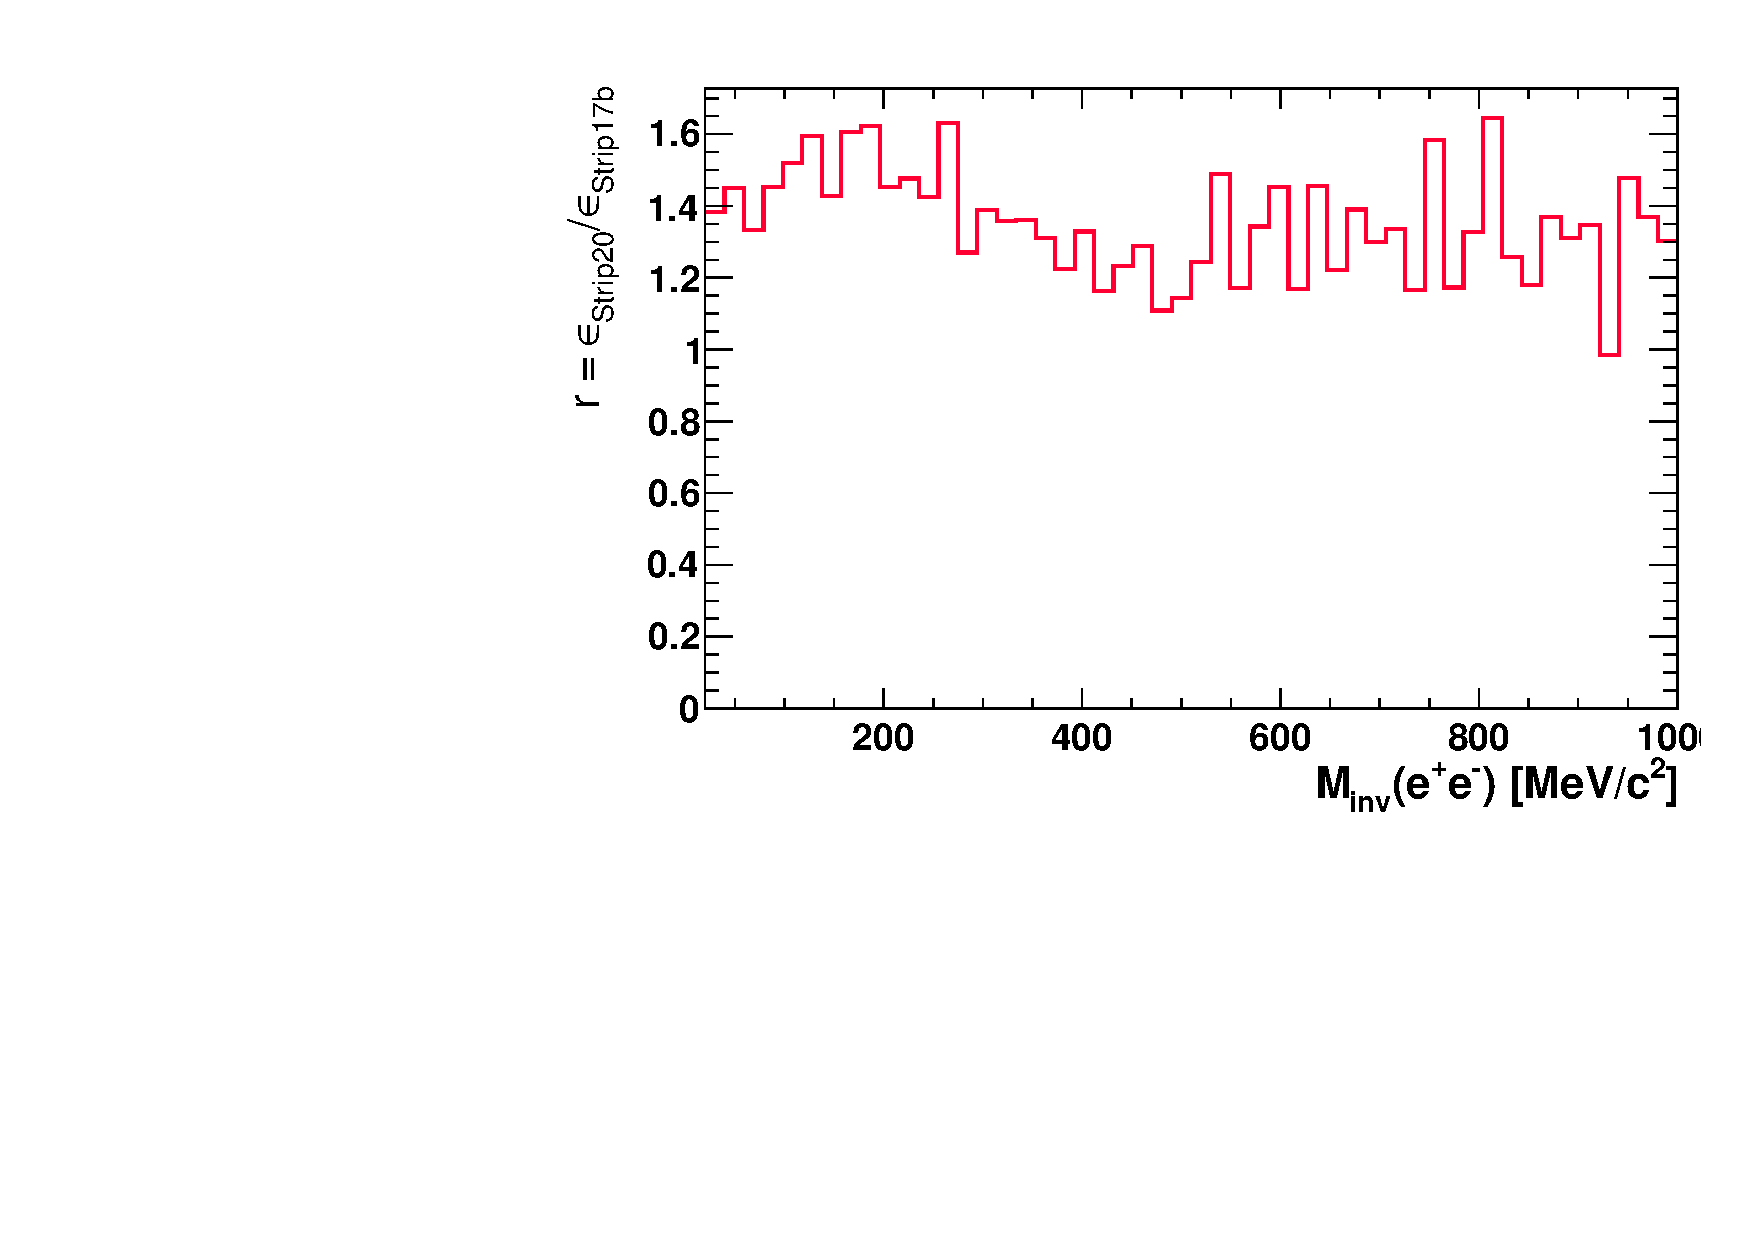
\includegraphics[width = 0.5\textwidth]{stripeff.pdf}
\end{center}
\vspace*{-0.5cm}
\caption{\textit{Ratio of efficiencies of the Stripping20 line with respect to the Stripping17b line for different bins of dielectron invariant mass.}}
\label{fig:stripeff}
\end{figure}
\\
The use of the \textit{Stripping20} line also implies the use of the \dielectronmaker (see Chapter \ref{chapter3}). As shown in Section \ref{sec:DiElectronMaker} this tool increases the resolution of the invariant dilepton mass. Therefore the lower cut on the invariant dilepton mass that was previously taken to be $M_{inv}(\epem)>30 \mevcc$ is now lowered to \\ $M_{inv}(\epem)>20 \mevcc$ without loss in precision.\newpage


\section{The Boosted Decision Tree selection}
Due to these changes the 2011 selection is not adapted to optimally select the \BdKstee candidates on the 2011 and 2012 data set. Therefore a completely new selection is developed and optimised.\\
In order to select the rare \BdKstee candidates a multivariate analysis (MVA) is used. The MVA is specially powerful in rejecting the so-called \textit{combinatorial background}, that is background that results from the false combination of tracks in the detector. The MVA chosen for this analysis is the Boosted Decision Tree (\bdtn) with gradient boost.\\
In this section the BDT is explained. Furthermore the data samples to train the \bdtn and the training strategy is summarised. At the end of this section the optimisation of the cut on the \bdtn classifier is shown.\\

\subsection{Boosted Decision Tree: a multivariate method}
\label{sec:bdt}
To separate the interesting signal events from the surplus of background events a set of $n$ discriminative variables is used. Classically each of these variables is examined independently of the others and a cut for each variable is found that rejects most of the background while keeping as much signal as possible. The total selection is then a rectangular set of $n$ cuts. \\
The multivariate analysis methods on the other hand combine the information on the different discriminate variables into one single classifier. The selection has then a linear or non-linear shape in the $n$-dimensional space of the variables. This principle is illustrated in Figure \ref{fig:zandra} \cite{zandri}.\\
\begin{figure}[ht]
\begin{center}
\vspace*{-0.5cm}
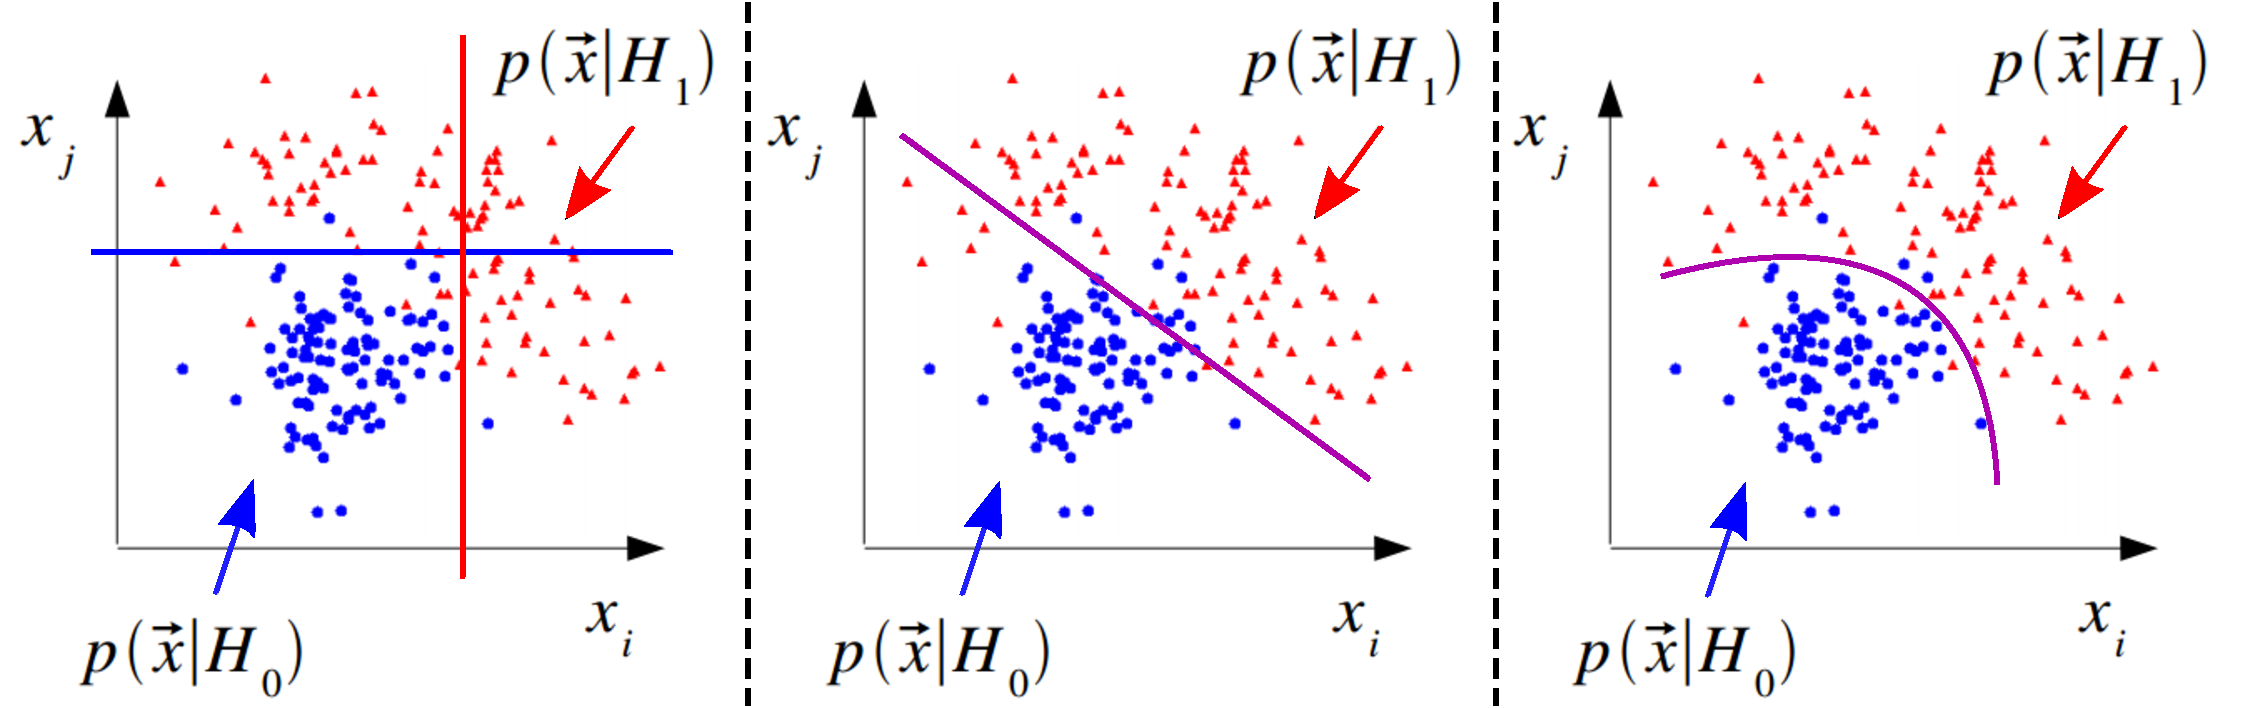
\includegraphics[width = 0.85 \textwidth]{zandra.pdf}
\end{center}
\caption{\textit{Illustration of the multivariate analysis for two variables $x_i$ and $x_j$ and two data types $H_0$ and $H_1$ (for example signal and background). The left plot shows a set of rectangular cuts as used in a classic selection. The middle and the right plot represent a selection from a multivariate analysis where the combination of variables is used to find the optimal selection. The middle plot shows a linear discriminant (Fischer discriminant) and the right plot shows a non-linear discriminant (Boosted Decision Tree, Neural Networks, etc.).}\cite{zandri}}
\label{fig:zandra}
\end{figure}

There are different multivariate methods of combining the variables to the final classifier and one of them is the Boosted Decision Tree. The \bdtn is a weighted sum of $m$ simple decision trees, called 'basic classifiers' or 'weak learners'. Each decision tree classifies a given event with $n$ variables $\mathbf{x}$ as either background or signal with the output of $f(\mathbf{x}) = -1$ and $f(\mathbf{x}) = 1$ respectively. The response $F(\mathbf{x})$ of the final \bdtn -- called the boosted event classification -- is then
\begin{equation}
F(\mathbf{x}) =\frac{1}{m} \sum_{i=0}^m \ln(\alpha_i) f_i(\mathbf{x})
\end{equation}
where the $\alpha_i$ represent the weights associated to the $i$th tree. Small values of $F(\mathbf{x})$ indicate that a certain events is more background-like while great values indicate a more signal-like structure.\\
\\
The \bdtn is trained on a sample of events that each have a label $y(\mathbf{x})$, meaning that they are already classified as signal or background.
During the training process, each decision tree aims at minimizing the weighted misclassification rate $err$. When training the first tree all events are given the same weight $\alpha = 1$. The subsequent tree $i$ is trained on a modified event sample where the previously misclassified events are given a weight derived from the previous misidentification rate $err_{(i-1)}$
\begin{equation}
\alpha_{i} = \frac{1 - err_{(i-1)}}{err_{(i-1)}}
\end{equation}
The entire sample is then renormalised such that the sum of the weights over all events remains normalised to 1.\\

\subsubsection{Gradient Boost}
The \bdtn used in this analysis implements the \textit{GradientBoost} method. This method is particularly good for selection of \BdKstee candidates since it performs very well in noisy environment, that is environment where some background events tend to look like signal. This is due to the fact that the loss-function (Equation \ref{eg:l}) varies smoothly and does not over-penalise misclassified events. As a consequence the \textit{GradientBosst} is very robust with respect to overtraining.\\
The \textit{GradientBoost} is a specialisation of the \bdtn. It works by implementing a \textit{loss-function} $L(F,y)$ which represents the deviation between the BDT response $F(\mathbf{x})$ and the true label $y(\mathbf{x})$ of a certain event. Furthermore, all events are given an individual weight corresponding to their loss-function. \\
The \textit{GradientBoost} implements a binomial log-likelihood loss
\begin{equation}
L(F,y) = \ln(1+e^{-2F(\mathbf{x})y})
\end{equation}
From here the average loss over the whole training sample with $k$ events can be calculated as
\begin{equation}
\langle L \rangle^{i} = \sum_{l=0}^k \omega^i_l L^i_l 
\label{eg:l}
\end{equation}
which is the analogon to the misclassification rate $err$. From $\langle L \rangle^{i}$ the boosting coefficient $\alpha_i$ for the $i$th tree can be computed
\begin{equation}
\alpha_i = \frac{\langle L \rangle^{i}}{1-\langle L \rangle^{i}}
\end{equation}
This boosting factor is used to extract the weight $\omega^i_k$ for each event $k$ in the $i$th step
\begin{equation}
\omega^i_k = \omega^{(i-1)}_k \cdot \alpha_i^{1-L^{(i-1)}_k}
\end{equation}
By minimizing the loss-function $ L^i(F(\mathbf{x}), y) $ in each step, that is for each decision tree, the total \bdtn is optimised.\\

\subsection{Strategy}
\label{sec:strategy}
The TMVA4 package implemented in \root is used for this analysis. As mentioned above all \bdtn were chosen to be of the type \textit{GradientBoost}.\\
The \bdtn requires training samples for the background and the signal. Unfortunately, the training samples cannot be used later on in the analysis because this would bias the selection. The \BdKstee decay has already a very small branching ratio and due to the low $p_T$ electrons the reconstruction efficiency is also low. It is crucial to keep as many events as possible for the analysis. However, the training sample for the \bdtn has to be large enough to compensate for statistical fluctuations.\\
To allow for the use of the entire data sample in the analysis while having enough statistics to train the \bdtn a strategy using two \bdts \ -- \bdta and \bdtb \ -- is developed. \bdta and \bdtb have the exact same properties the only difference being the data samples they are trained on. For the training the data sample is divided into four independent subsamples of equal size as shown in Figure \ref{fig:samples}. The sample A1 is used to train the \bdta and B1 is used to train \bdtb . The testing and the optimisation is executed on A2 and B2 for \bdta and \bdtb respectively. \\
\begin{figure}[ht]
\begin{center}
\vspace*{-0.5cm}
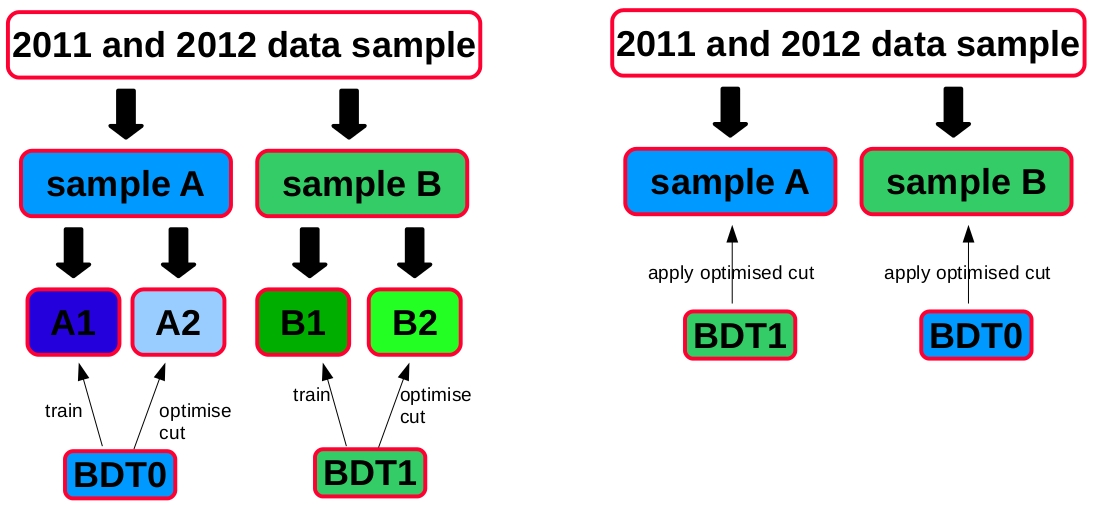
\includegraphics[width = 0.8\textwidth]{BDTstrategy.jpg}
\end{center}
\caption{\textit{Schematic illustration of the division of the data sample into four subsamples to train the \bdts and optimise the cut on \bdta and \bdtb.}}
\label{fig:samples}
\end{figure}

For the final selection, the \bdta is applied on the data sample B and the cut that was optimised on the data sample A2 is performed. In return the \bdtb and its cut optimised on the B2 sample are applied to the entire data sample A. Hereby is ensured that the entire data sample can be used in the analysis without any bias from the training procedure.\\
While this procedure has been developed for the \lhcb data sample specifically, it is also applied on the Monte Carlo signal sample to ensure equal treatment of the background and signal sample.\newpage

\subsection{The input variables}
\label{sec:variables}
The variables for the \bdtn must have discriminative power between the combinatorial background and the \BdKstee signal.\\
The tracks originating from \Bd mesons have a distribution of transverse momentum $p_T$ that is greater than for tracks that do not come from a \Bd meson. This is due to the fact that \Bd mesons are relatively heavy. Due to the large \Bd lifetime, the impact parameter significance with respect to the primary vertex of the tracks originating from the \Bd decay is much larger than those of tracks from combinatorial background. Furthermore the quality of the vertices in events that are combinatorial background is lower because the tracks do not really originate from the same vertices. Therefore the interesting variables are the significance of the impact parameter $\chi^2_{IP}$ for all particles, the significance of the decay vertices $\chi^2_{Vertex}$ of the \Bd, the \Kstarz and the (\epem), the flight distance significance $\chi^2_{FD}$ of the \Bd, the \Kstarz and the (\epem) and the $\theta_{flight}$\footnote{As mentioned in the previous section, $\theta_{flight}$ is the angle between the direction of the \Bd candidate momentum and the direction between the primary vertex and the \B decay vertex.} of the \Bd meson. All input variables are listed in Table \ref{tab:newbdt} and a selection of these variables is plotted in Figure \ref{fig:variables} for background and signal respectively (plots of all variables can be found in Appendix \ref{ap:allvars}).\\
\begin{figure}[ht]
\vspace*{-0.5cm}
\begin{center}
\centering
\subfigure{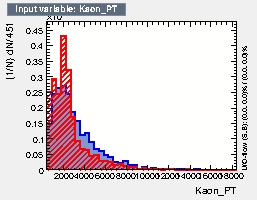
\includegraphics[width = 0.45 \textwidth]{kaonpt.jpg}}
\centering
\subfigure{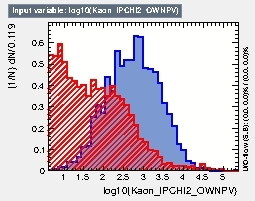
\includegraphics[width = 0.45 \textwidth]{kaonipchi2.jpg}}
\subfigure{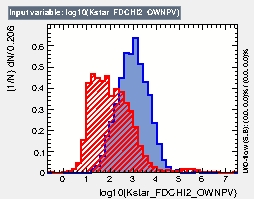
\includegraphics[width = 0.45 \textwidth]{kstarfdchi2.jpg}}
\subfigure{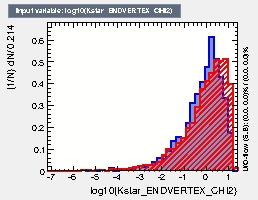
\includegraphics[width = 0.45 \textwidth]{kstarendvertex.jpg}}
\end{center}
\caption{\textit{A choice of variables used in the \bdtn training. The red distribution represents the combinatorial background while the blue distribution comes from the signal. \textbf{Top left:} \kaon transverse momentum $p_T(\kaon)$, \textbf{top right:} logarithm of \kaon impact parameter significance $log(\chi^2_{IP}(\kaon))$, \textbf{bottom left:} logarithm of \Kstarz flight distance significance $log(\chi^2_{FD}(\Kstarz))$, \textbf{bottom right:} logarithm of \Kstarz vertex quality $log(\chi^2_{Vertex}(\Kstarz))$. }}
\label{fig:variables}
\end{figure}

\begin{table}[ht]
\vspace*{-0.5cm}
\begin{center}
\begin{tabular}{c|l}
Particle & Variable \\
\hline
\hline
 \Bd & $p_T$,\qquad $log(\chi^2_{IP})$,\qquad $log(\chi^2_{FD})$,\qquad $log(\chi^2_{Vertex})$,\qquad $\theta_{flight}$ \\
\hline 
\Kstarz & $p_T$,\qquad $log(\chi^2_{IP})$,\qquad $log(\chi^2_{FD})$,\qquad $log(\chi^2_{Vertex})$ \\
\hline 
(\epem) & $p_T$,\qquad $log(\chi^2_{IP})$,\qquad $log(\chi^2_{FD})$,\qquad $log(\chi^2_{Vertex})$ \\
\hline
\kaon & $p_T$,\qquad $log(\chi^2_{IP})$ \\
\hline
\pion & $p_T$,\qquad $log(\chi^2_{IP})$ \\
\hline
\ep & $p_T$,\qquad $log(\chi^2_{IP})$ \\
\hline
\en & $p_T$,\qquad $log(\chi^2_{IP})$ \\
\hline
& number of primary vertices $nPV$
\end{tabular}
\caption{\textit{Variables used in the Boosted Decision Trees \bdta and \bdtb .}}
\label{tab:newbdt}
\end{center}
\end{table}
\vspace*{-0.5cm}
Additionally the number of primary vertices $nPV$ is used as variable in the training. It can be shown, that the distributions of some of the above variables differ for the background depending on $nPV$. Figure \ref{fig:npvvariation} shows an example. This is due to the fact, that events with $nPV = 1 $ are very likely to have come from a real \B meson in order to pass the stripping. Therefore the distribution of the discriminant variables for the background is more similar to the distribution from the signal. Events with several primary vertices are more likely to form combinatorial background that passes the selection due to the track multiplicity in the detector. Since these events do not come from a real \B meson, their distributions in the discriminant variables differ more from the signal. Including $nPV$ in the analysis allows to take into account the differing distributions of the other variables and the fact that events with high $nPV$ have a greater probability to be combinatorial background.\\
\begin{figure}[!h]
\vspace*{-0.5cm}
\begin{center}
\subfigure{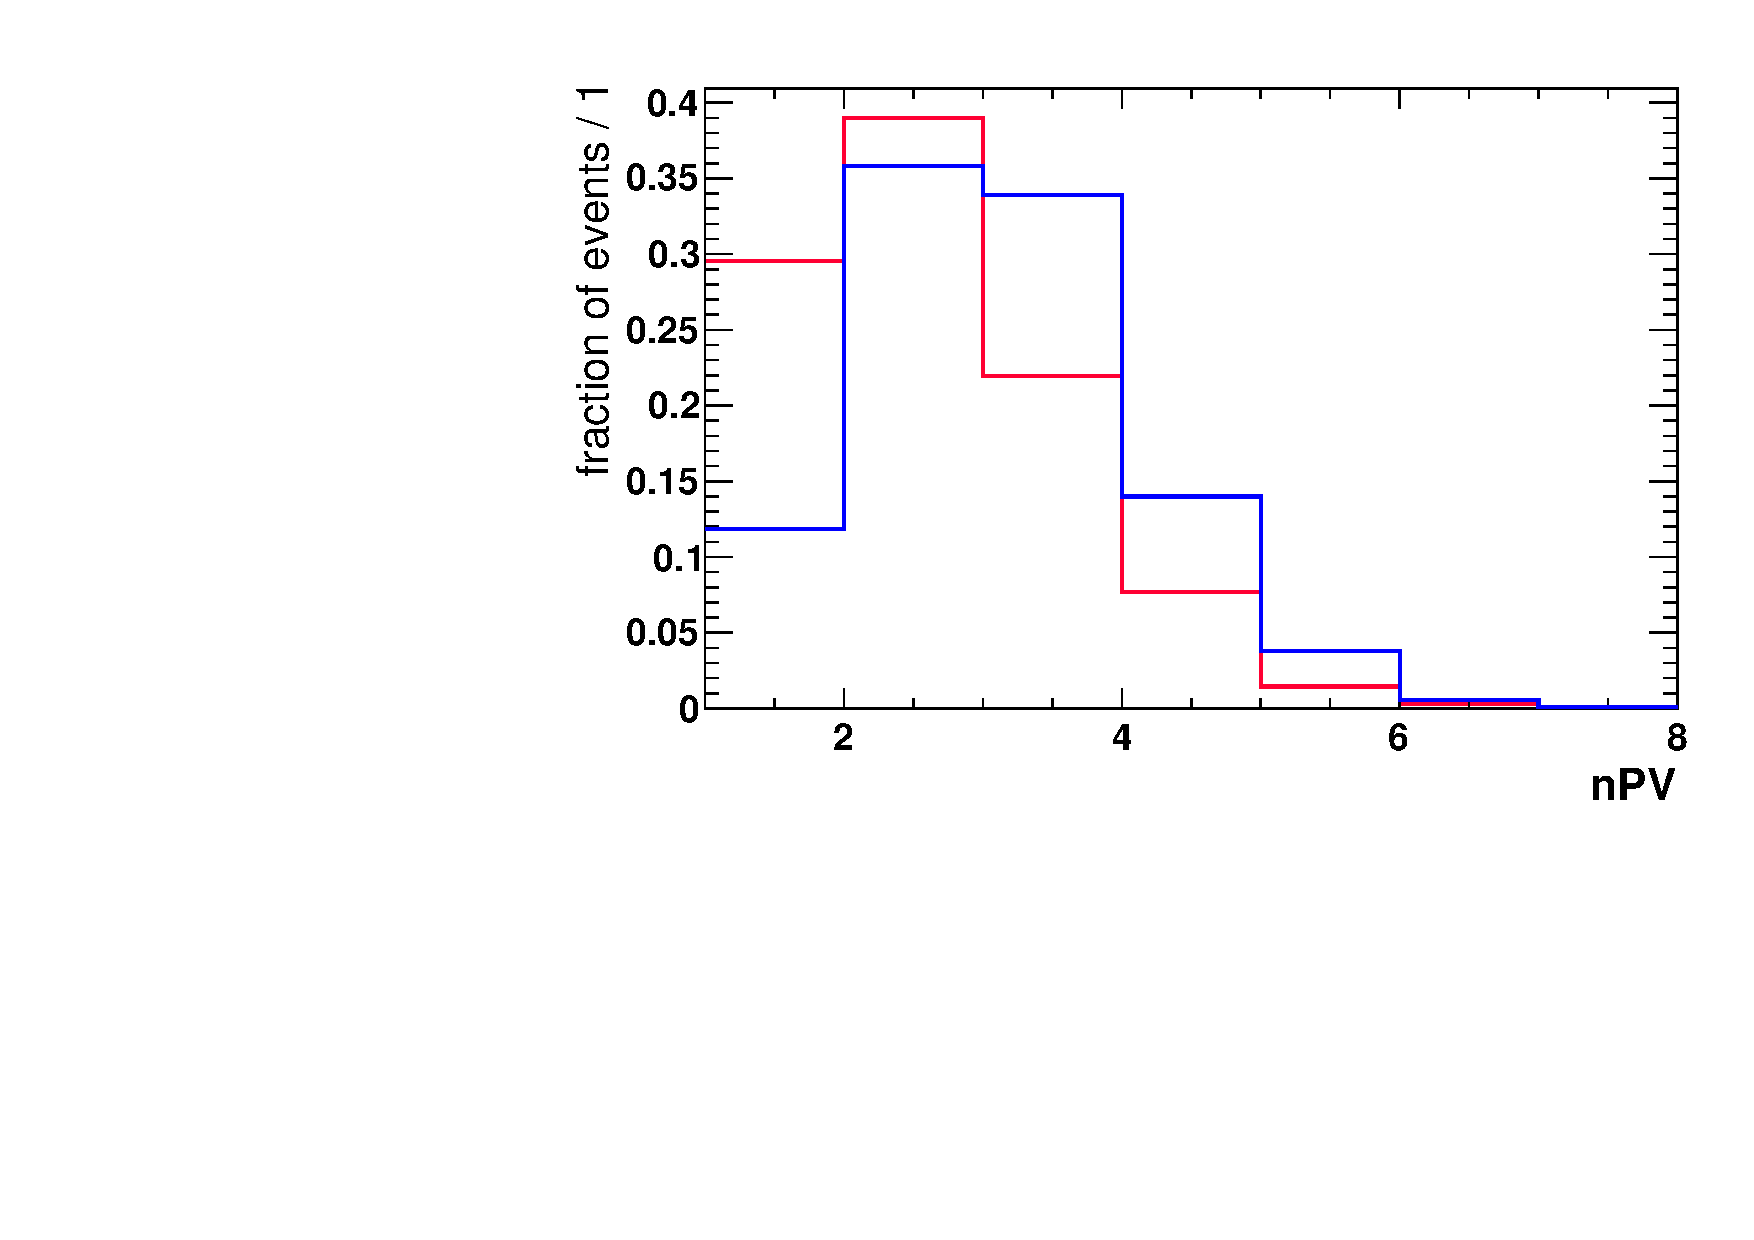
\includegraphics[width=0.48\textwidth]{nPV_eeKstar.pdf}}
\subfigure{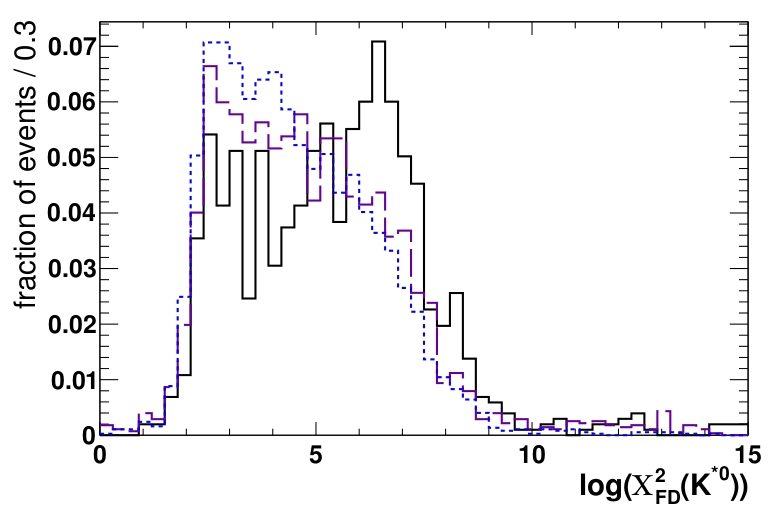
\includegraphics[width=0.51\textwidth]{nPV_Kstar_FDCHI2.jpg}}
\end{center}
\vspace*{-0.8cm}
\caption{\textit{\textbf{Left:} Normalized distribution of the number of primary vertices for the signal (pink) and the combinatorial background (blue). \textbf{Right:} Illustration of how the distribution of a variable varies with the number of primary vertices. The plot shows the normalized distributions of the logarithm of the \Kstarz flight distance significance. Black distribution: nPV = 1, blue distribution: nPV = 2, violet distribution: nPV>2. These distributions have been obtained from a sample for combinatorial background from \lhcb data.}}
\label{fig:npvvariation}
\end{figure}
Despite their discriminate power the particle identification variables $\mathrm{DLL}$ (see Section \ref{sec:pid}) are not included in the training as their distributions are not well reproduced in the Monte Carlo. They will, however, later be used in the optimisation of the selection.\\

\subsection{The data samples for the \bdtn training}
In this section the data samples used in the \bdtn training are discussed. The sample representing the background is taken from \lhcb data while the signal sample comes from \BdKstee Monte Carlo. Both samples have been processed by the \BdKstee \textit{Stripping20} line and reconstructed in \davinci v33 including the DiElectronMaker (see Chapter \ref{chapter3}). After the stripping a rough preselection that will be discussed in the next section is applied before training the \bdtn.\\
The statistics of the training samples is limited by the available amount of background \lhcb data. This results in training samples of the size of $\approx$3300 events for each \bdtn and for signal and background respectively.\\

\subsubsection{The preselection}
\label{sec:presel}
The preselection is a set of cuts dedicated to removing events that have a very small probability of being \BdKstee candidates. Additionally to the cuts listed in Table \ref{tab:presel} the candidates are asked to be either in the \textit{L0ElectronTOS}, \textit{L0HadronTOS} or \textit{L0TIS} category (see Section \ref{sec:req} for definition) and were triggered by the \textit{Hlt1TrackAllL0Decision} and one of the the \textit{\hlttwo topological lines} (see Section \ref{sec:hlt} for more details).\\
\begin{table}[ht]
\vspace*{-0.5cm}
\begin{center}
\begin{tabular}{c|c}
Particle & Cut \\
\hline
\hline
\Kstarz & $| m(\Kstarz ) -892 \mevcc | \, < \, 100 \mevcc$ \\
\hline
(\epem) & $20 \mevcc \, < \, m(\epem) \, < 1000 \mevcc $\\
\hline
\kaon & $\dllkpi\, > \, 0$ \\
\hline
\pion & $\dllkpi\, < \, 5$ \\
\hline
\epm & $\dllepi \, >\, 0$\\
\end{tabular}
\caption{\textit{Preselection cuts for the \BdKstee analysis.}}
\label{tab:presel}
\end{center}
\end{table}
\vspace*{-0.4cm}
\subsubsection{The \BdKstee signal sample}
\label{sec:splot}
The signal sample for the \bdtn is taken from \BdKstee Monte Carlo. Unfortunately the distribution of number of primary vertices ($nPV$) is not well simulated in the Monte Carlo. To obtain a accurate training of the \bdtn the distribution of $nPV$ has to be reweighted to match the distribution of $nPV$ of the \BdKstee signal on \lhcb data. Therefore the $nPV$ distribution of the signal on \lhcb data has to be extracted and compared to the Monte Carlo $nPV$ distribution. This can be done by using a statistical tool called the the sPlot technique \cite{splot}. \\
\newpage
\textbf{The sPlot technique}\\
The sPlot technique can extract the contribution of the signal to the distribution of a variable $x$ when the signal is not clearly separable from the background. First the distribution of the variable $x$ in the signal window (where signal and background are mixed) is extracted. Then the distribution of $x$ in the region where only background contributes is taken. By calculating the contribution for the background in the signal window, the background-only distribution of $x$ can be subtracted from the signal-background distribution, leaving the distribution of the variable $x$ for the signal decay only.\\
\\
\textbf{Implementation of the sPlot technique}\\
There are not enough signal events in the \BdKstee data sample from 2011 and 2012 to apply the sPlot technique. The \BdToJPsieeKst decay on the other hand has a $ \BR(\BdToJPsieeKst) = 1.34 \cdot 10^{-3} $ which is two orders of magnitude higher and and provides enough statistics to use the sPlot tool implemented in \root.\\
In general the $nPV$ distribution should be independent of the specific decay. But the selection procedure can distort the distribution, particularly there is a cut on the hit multiplicity in the \spd (Section \ref{sec:lhcb}) in the L0 trigger lines. This relates to the number of primary vertices. Nevertheless it is convenient that the \BdToJPsieeKst decay shows the same kinematics as the \BdKstee decay.\\
To extract the correct $nPV$ distribution the \BdToJPsieeKst candidates experience the same reconstruction and selection procedure as the \BdKstee candidates. This is done by taking the output of the \BdKstee \textit{Stripping20} line\footnote{The \BdKstee \textit{Stripping20} line was developed to reconstructed \BdKstee candidates with low $m(\epem)$ but there is no explicit cut on $m(\epem)$ and \BdToJPsieeKst candidates are reconstructed as well.} and applying the same preselection cuts as above with the difference of performing a cut on the mass of the \jpsi of $2400 \mevcc \, < \, m(\jpsi) \, < 3400 \mevcc $.\\
Using the \BdToJPsieeKst decay has another advantage because the \jpsi is a narrow resonance. For the sPlot technique the mass of the \jpsi is fixed to the PDG value $m(\jpsi) = 3096 \mevcc$. From there the electron momenta are recalculated and finally the \Bd mass is recalculated. The fixing of the \jpsi mass yields a more narrow signal peak as can be seen in Figure \ref{fig:jpsi}.\\
The sPlot tool in \root is given the \BdToJPsieeKst candidates along with a probability distribution function (\PDF) for the signal and the background respectively. The signal \PDF was taken to be a double Crystal-Ball distribution (CB) \cite{crystal} with both CBs sharing the same $\mu_{\B}$, $\alpha$ and $n$. All variables of the signal \PDF are determined by a fit to the \BdToJPsieeKst Monte Carlo, except for the \Bd mass. The widths $\sigma_1$ and $\sigma_2$ are free to scale about the same factor. The background shape was assumed to be exponential. The fit to the constrained \Bd mass can be seen in Figure \ref{fig:jpsi}.\\
\\
The extracted $nPV$ distribution is shown in Figure \ref{fig:npv} along with the distribution from Monte Carlo and the reweighted Monte Carlo distribution. From here the $nPV$ distribution from \BdKstee Monte Carlo is reweighted in the same way.
\begin{figure}[ht]
\vspace*{-0.5cm}
\begin{center}
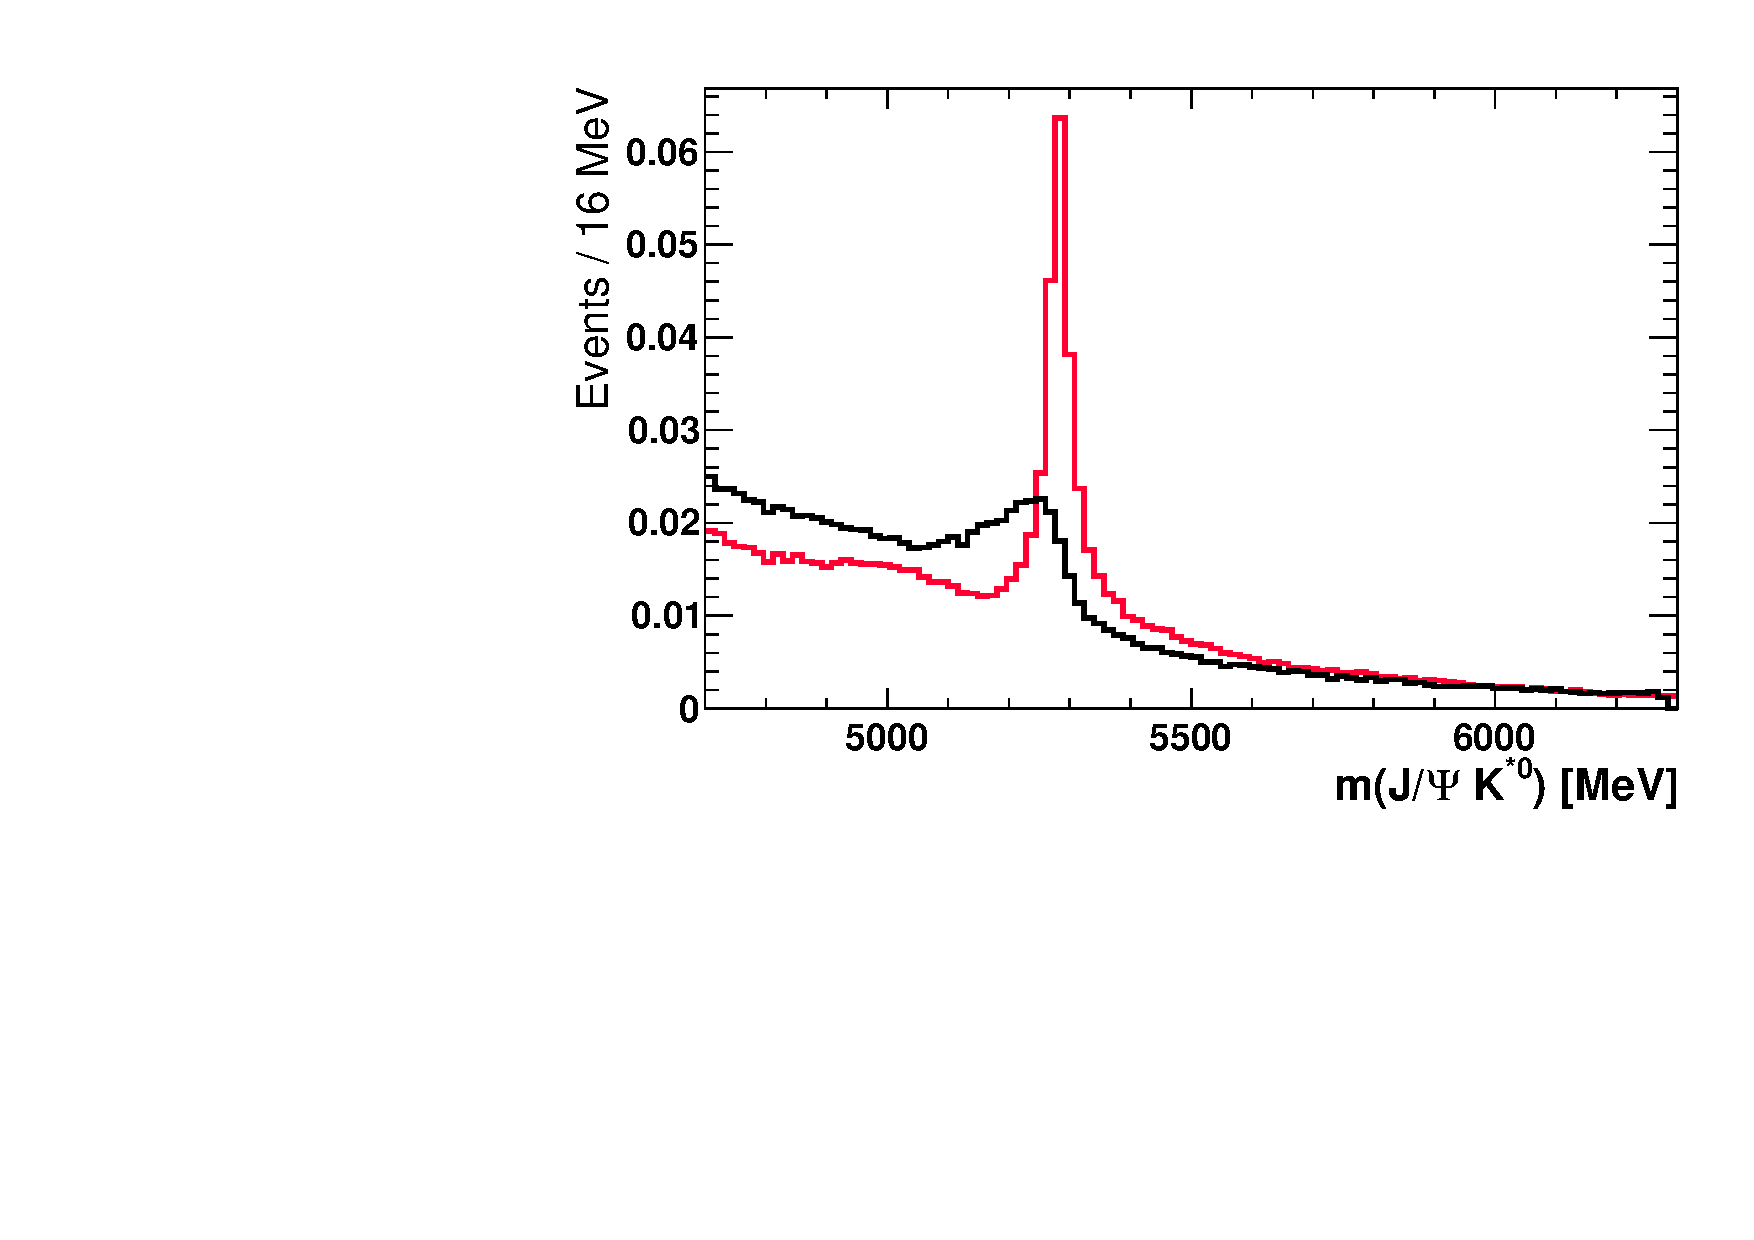
\includegraphics[width = 0.5 \textwidth]{mB_Jpsi.pdf}
\end{center}
\vspace*{-0.8cm}
\caption{\textit{The $m(e^{+}e^{-}K^{*0})$ mass distribution of the 2011 and 2012 \lhcb data from the Stripping20 \BdToJPsieeKst line after preselection (Section \ref{sec:presel}). The black distribution is the normal \Bd mass distribution, the pink distribution is with the constrained \jpsi mass fixed to the PDG value.}}
\label{fig:jpsi}
\end{figure}

\begin{figure}[ht]
\begin{center}
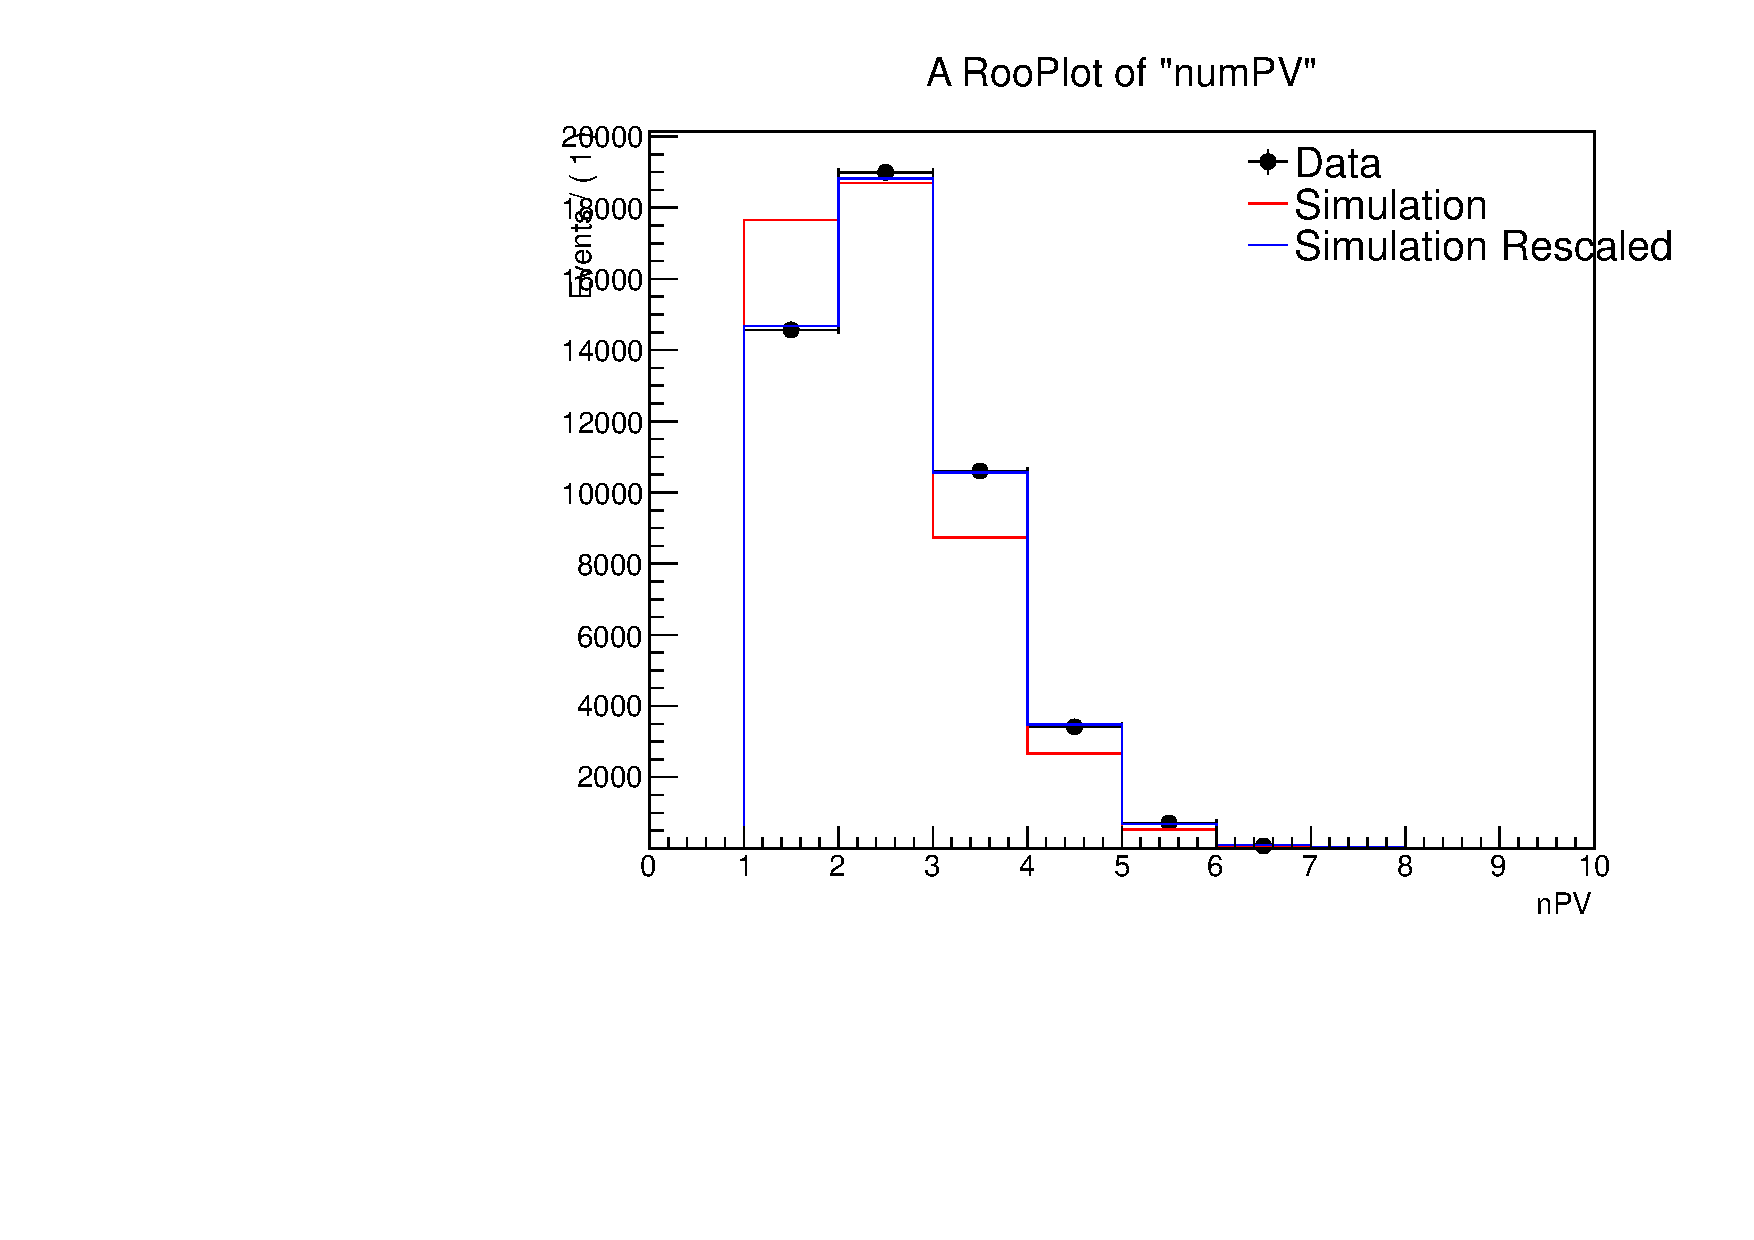
\includegraphics[width = 0.5 \textwidth]{nPV.pdf}
\end{center}
\vspace*{-0.8cm}
\caption{\textit{The $nPV$ distribution for the \BdToJPsieeKst candidates. Black points: signal from \lhcb data, red distribution: Monte Carlo, blue distribution: reweighted Monte Carlo.}}
\label{fig:npv}
\end{figure}


\subsubsection{The background sample}
The \bdtn is very effective against combinatorial background and should hence be trained on combinatorial background only. Therefore the data for the background is taken to be the upper sideband of the 2011 and 2012 data sample as shown in Figure \ref{fig:sb}.
\begin{figure}[ht]
\vspace*{-0.5cm}
\begin{center}
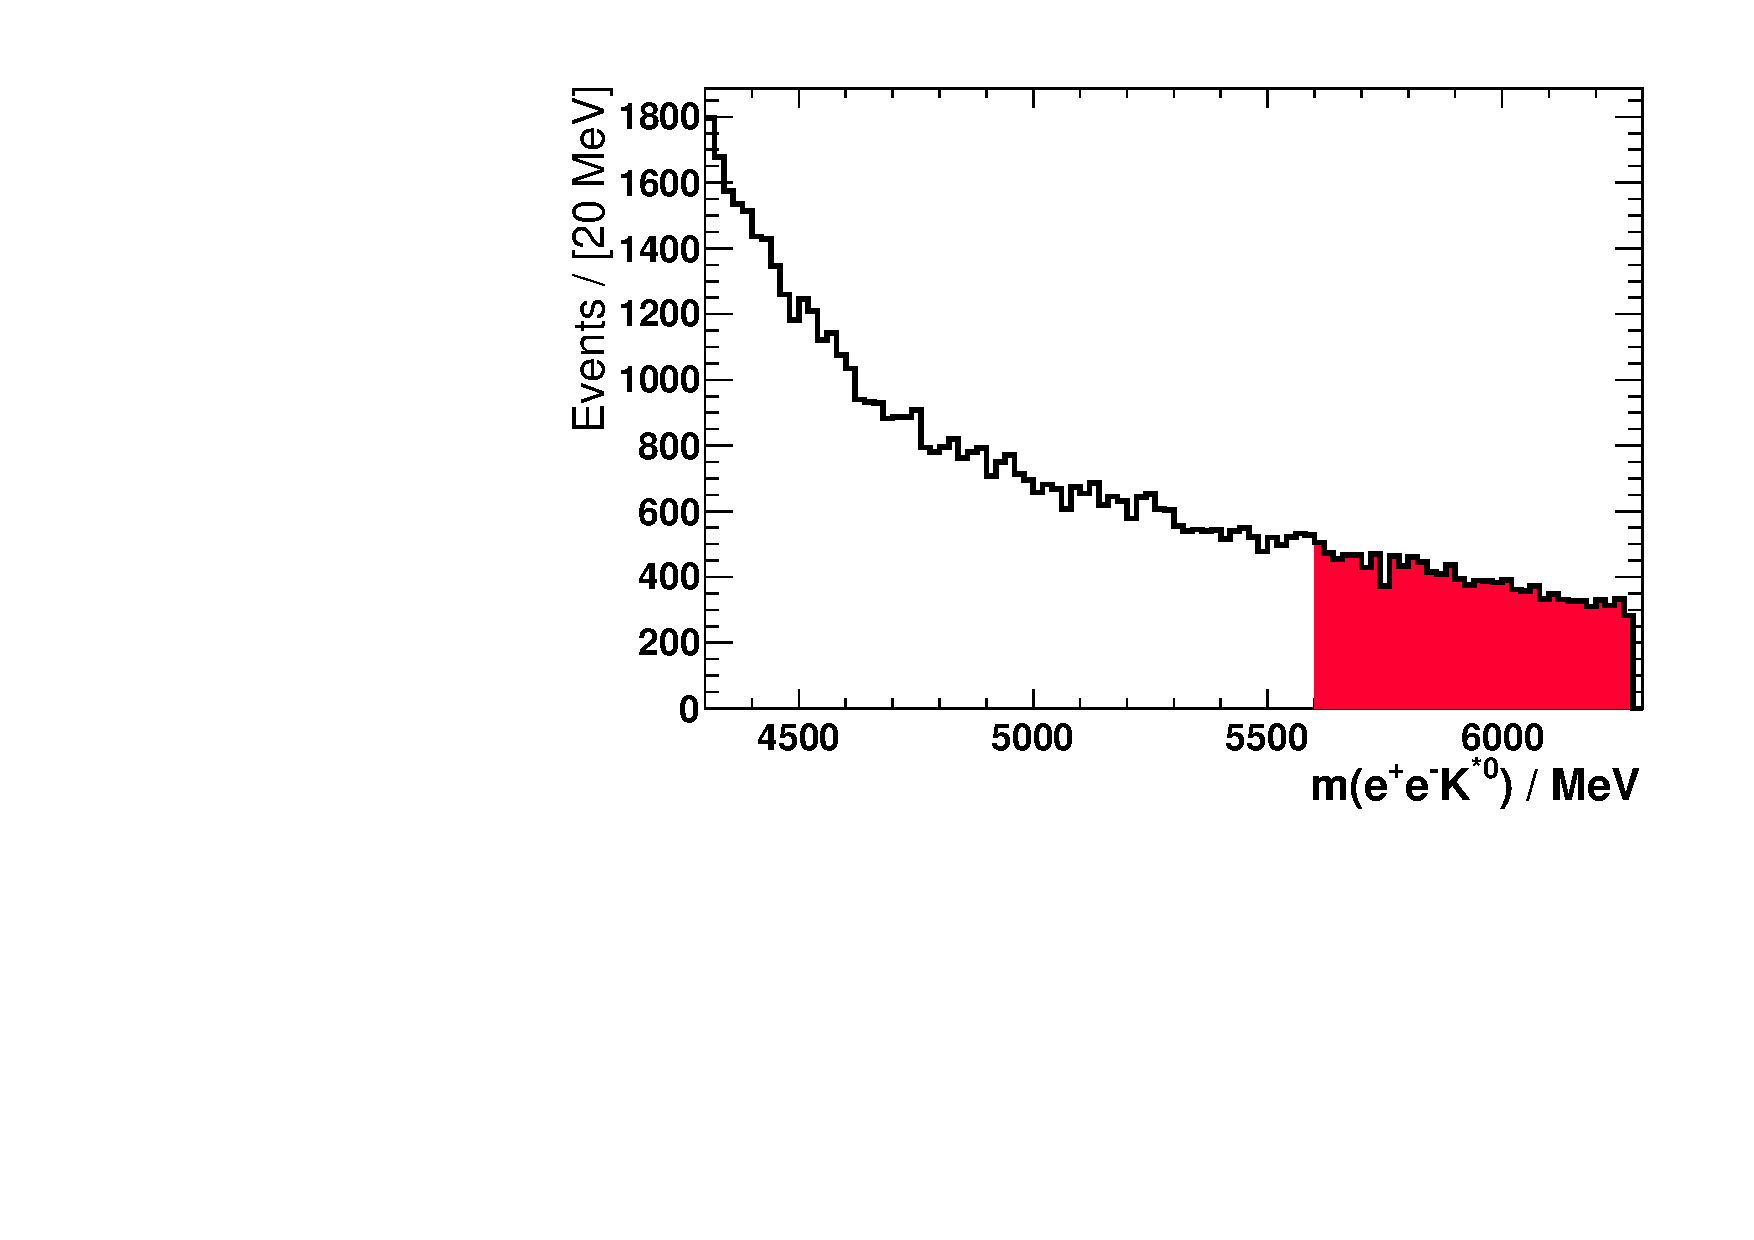
\includegraphics[width = 0.4 \textwidth]{upperSideBand.pdf}
\end{center}
\vspace*{-0.8cm}
\caption{\textit{The $m(e^{+}e^{-}K^{*0})$ mass distribution of the 2011 and 2012 \lhcb data from the \BdKstee Stripping20 line after preselection (Section \ref{sec:presel}). The pink distribution represents the candidates used in the training of the \bdts.}}
\label{fig:sb}
\end{figure}

\subsection{Results of the \bdtn trainings}
The response of \bdta and \bdtb after the training is shown in Figure \ref{fig:BvsS} and Figure \ref{fig:resp}. Figure \ref{fig:BvsS} shows the background rejection efficiency as a function of the signal selection efficiency obtained from applying the trained \bdts on the testing samples.\\
Figure \ref{fig:resp} shows the response of the trained \bdts on the signal and the background. It can be seen from the accordance of the distributions of the testing and the training samples that the \bdts were not overtrained. Furthermore it was tested if the response of the \bdts on the data is well reproduced by the Monte Carlo. The extraction of the \bdtn response of the \lhcb signal was done using the \BdToJPsieeKst decay and the sPlot technique just as explained in Section \ref{sec:splot}. The results are displayed in Figure \ref{fig:comp} and show that the distributions from Monte Carlo and \lhcb signal are in reasonable agreement with each other. \\
\begin{figure}[ht]
\vspace*{-0.2cm}
\begin{center}
\subfigure{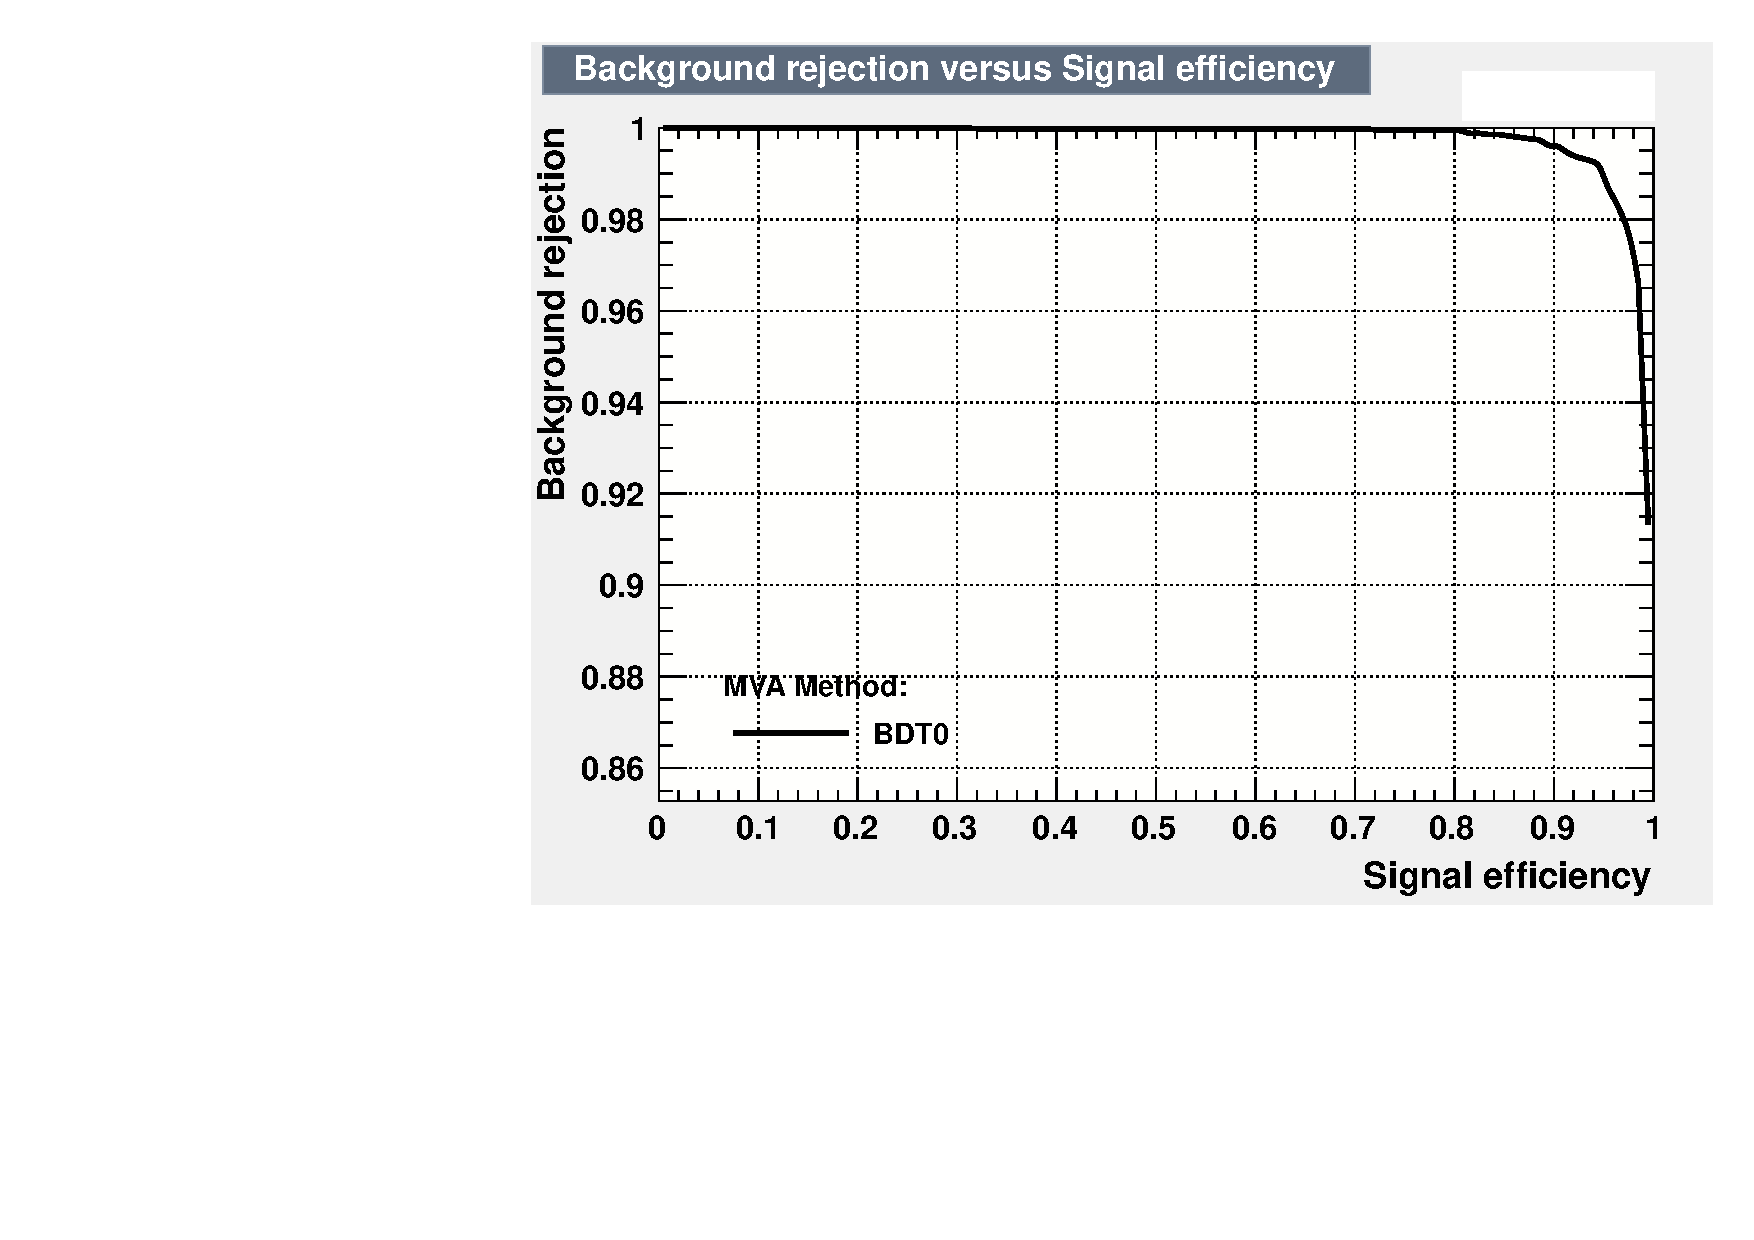
\includegraphics[width = 0.49 \textwidth]{BDT0_ROC.pdf}}
\subfigure{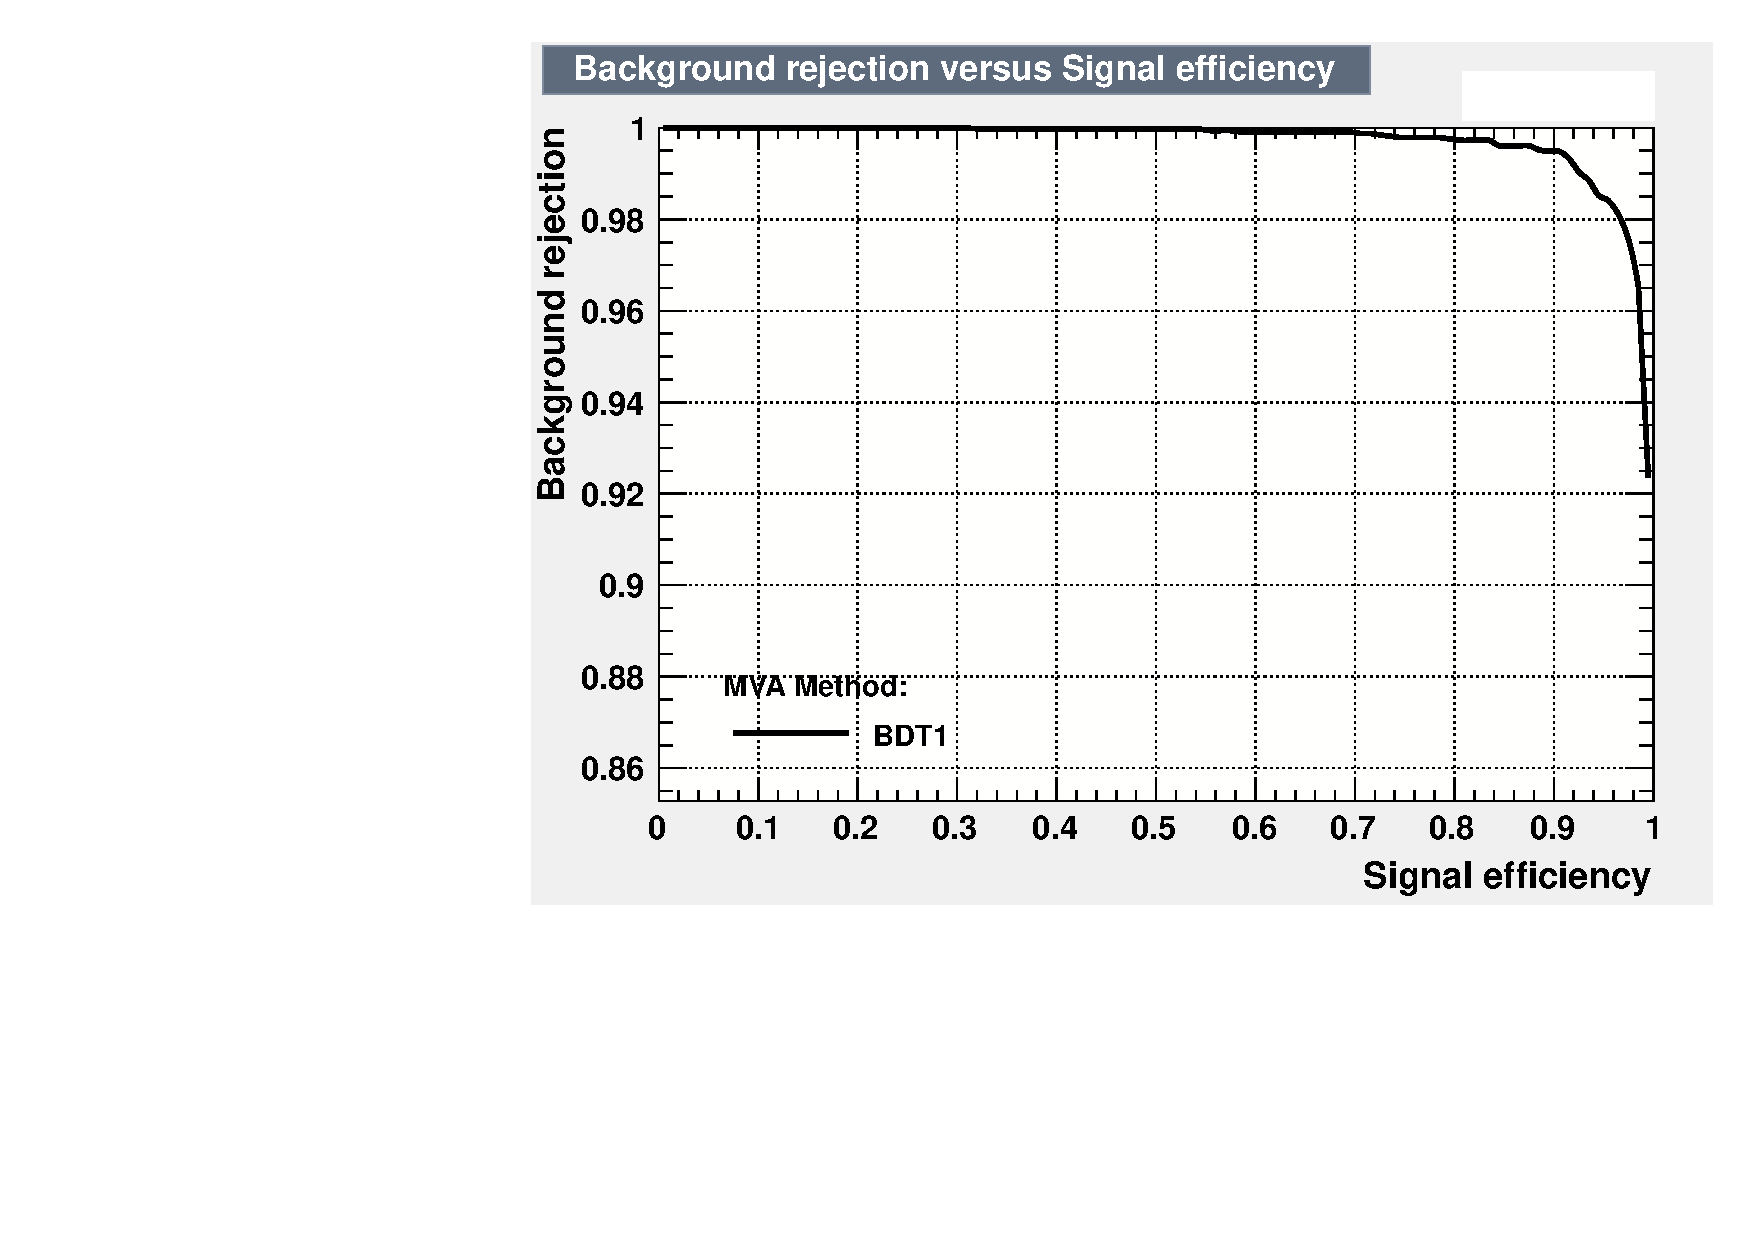
\includegraphics[width = 0.49 \textwidth]{BDT1_ROC.pdf}}
\end{center}
\vspace*{-0.8cm}
\caption{\textit{Background rejection efficiency as a function of the signal selection efficiency for the trained \bdta (left) and the \bdtb (right).}}
\label{fig:BvsS}
\end{figure}

\begin{figure}[ht]
\begin{center}
\subfigure{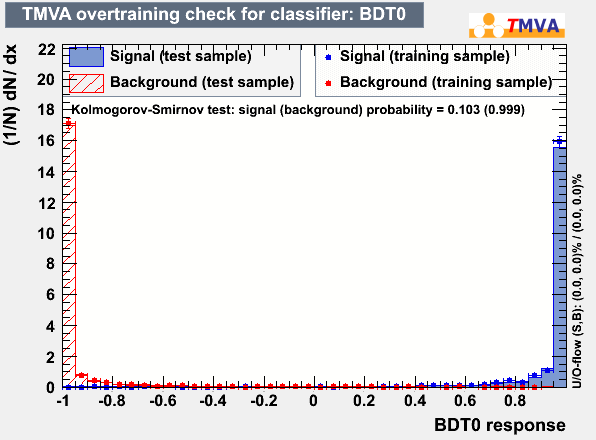
\includegraphics[width = 0.49 \textwidth]{responsea.png}}
\subfigure{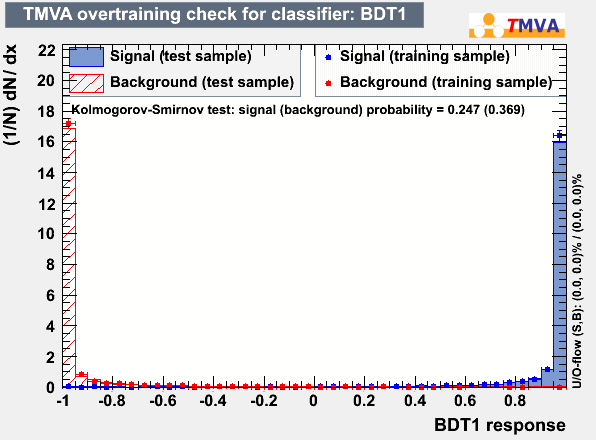
\includegraphics[width = 0.49 \textwidth]{responseb.png}}
\end{center}
\vspace*{-0.8cm}
\caption{\textit{\bdtn response on the signal and the background. Red dots: response on the background training sample, red area: response on the background testing sample, blue dots: response on the signal training sample, blue area: response on the signal testing sample. The response for the testing and the training samples coincide for signal and background respectively which shows that \bdts were not overtrained.}}
\label{fig:resp}
\end{figure}

\begin{figure}[ht]
\begin{center}
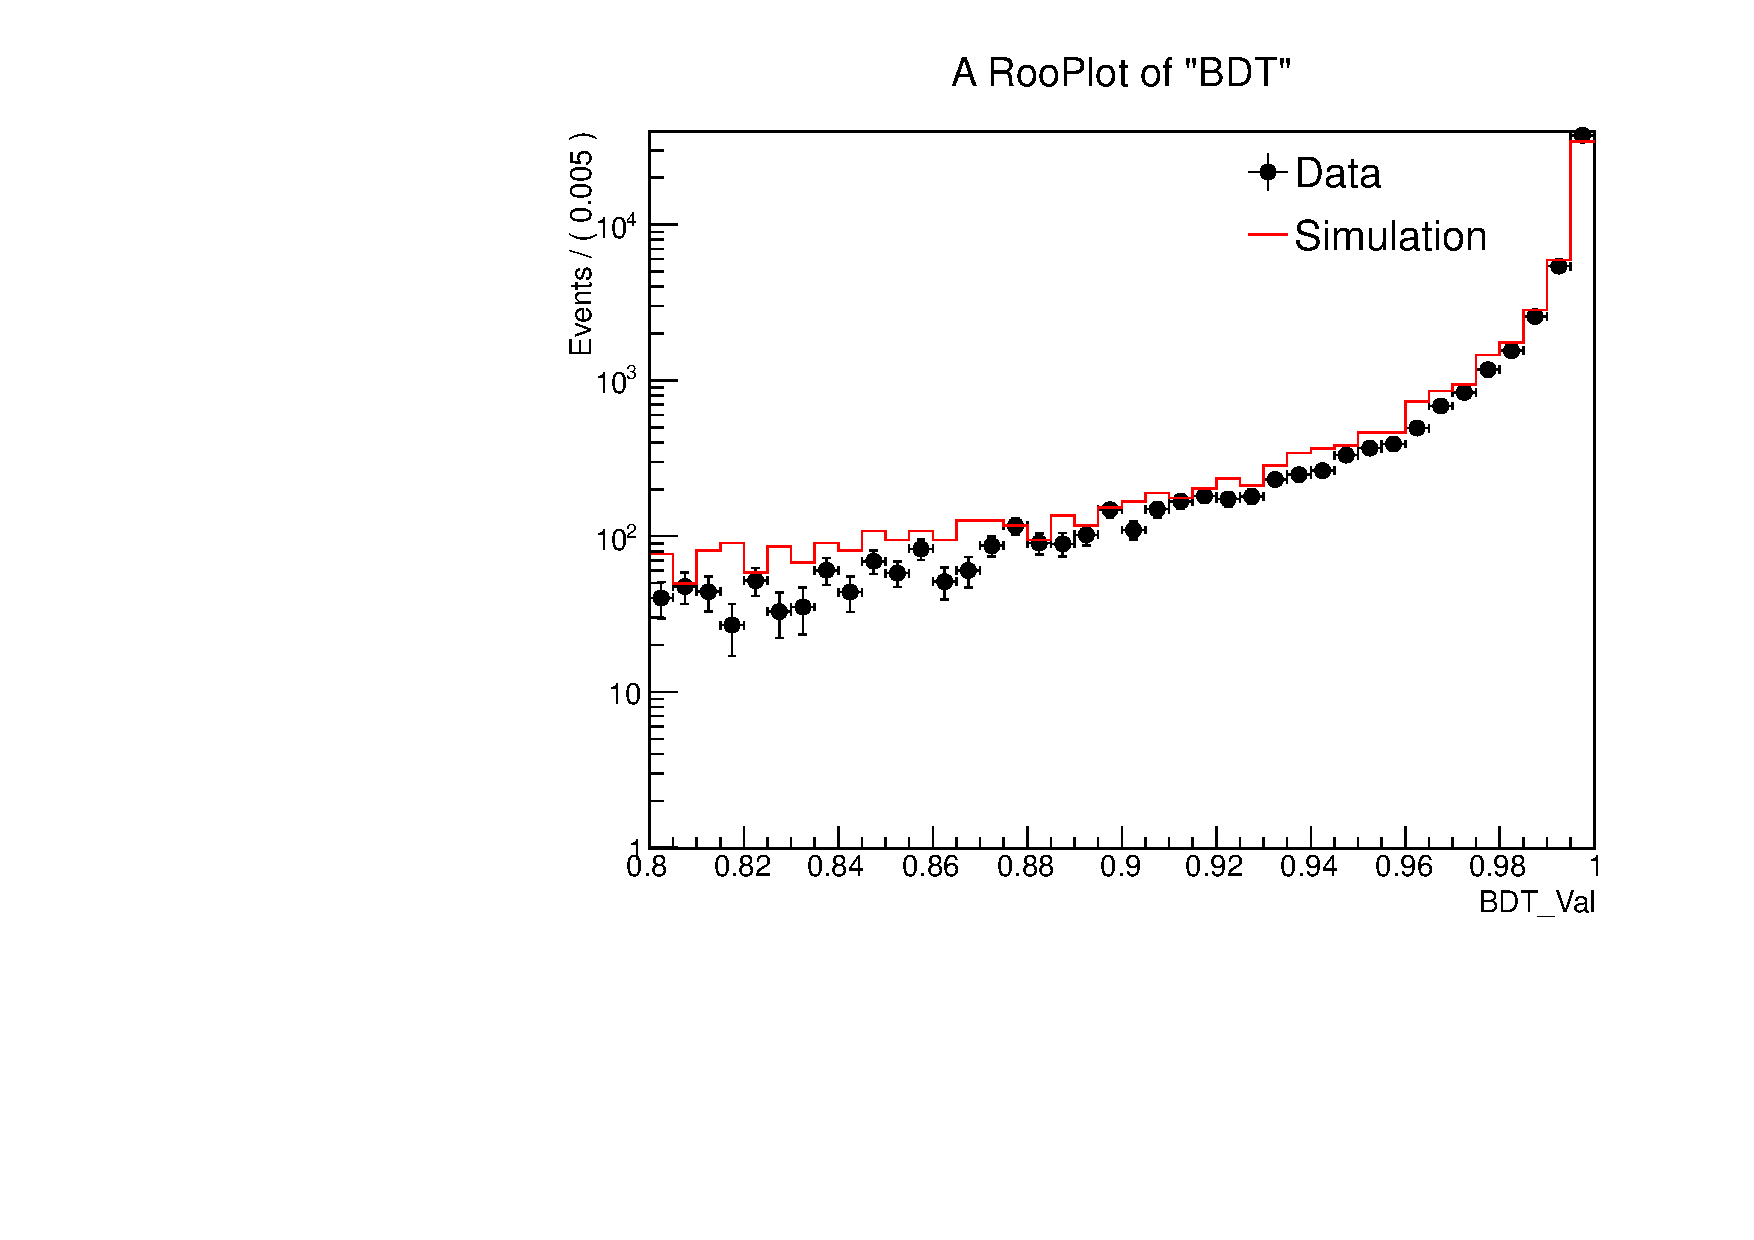
\includegraphics[width = 0.49 \textwidth]{BDT_comp.pdf}
\end{center}
\vspace*{-0.5cm}
\caption{\textit{Distribution of the \bdtn response on the \BdToJPsieeKst Monte Carlo (red curve) and \BdToJPsieeKst \lhcb data (black dots) in the region around the working point of the \bdtn cut.}}
\label{fig:comp}
\end{figure}

In order to compare the behaviour of \bdta and \bdtb both are applied to all events in the \BdKstee Monte Carlos and the \lhcb data after the preselection. Figure \ref{fig:bdtvsbdt} shows the average value of \bdtb for a given bin of \bdta  value on data as well as Monte Carlo. Due to the limited amount of Monte Carlo events below a \bdtn value < 0.5 the points below this value are not representative. Above 0.8 -- the region in which the working point will lie -- the points show the same systematics for Monte Carlo and data respectively. This behaviour reflects the coherence between \bdta and \bdtb. The deviance from the diagonal is the result of statistical fluctuations in the training samples.

\begin{figure}[ht]
\begin{center}
\subfigure{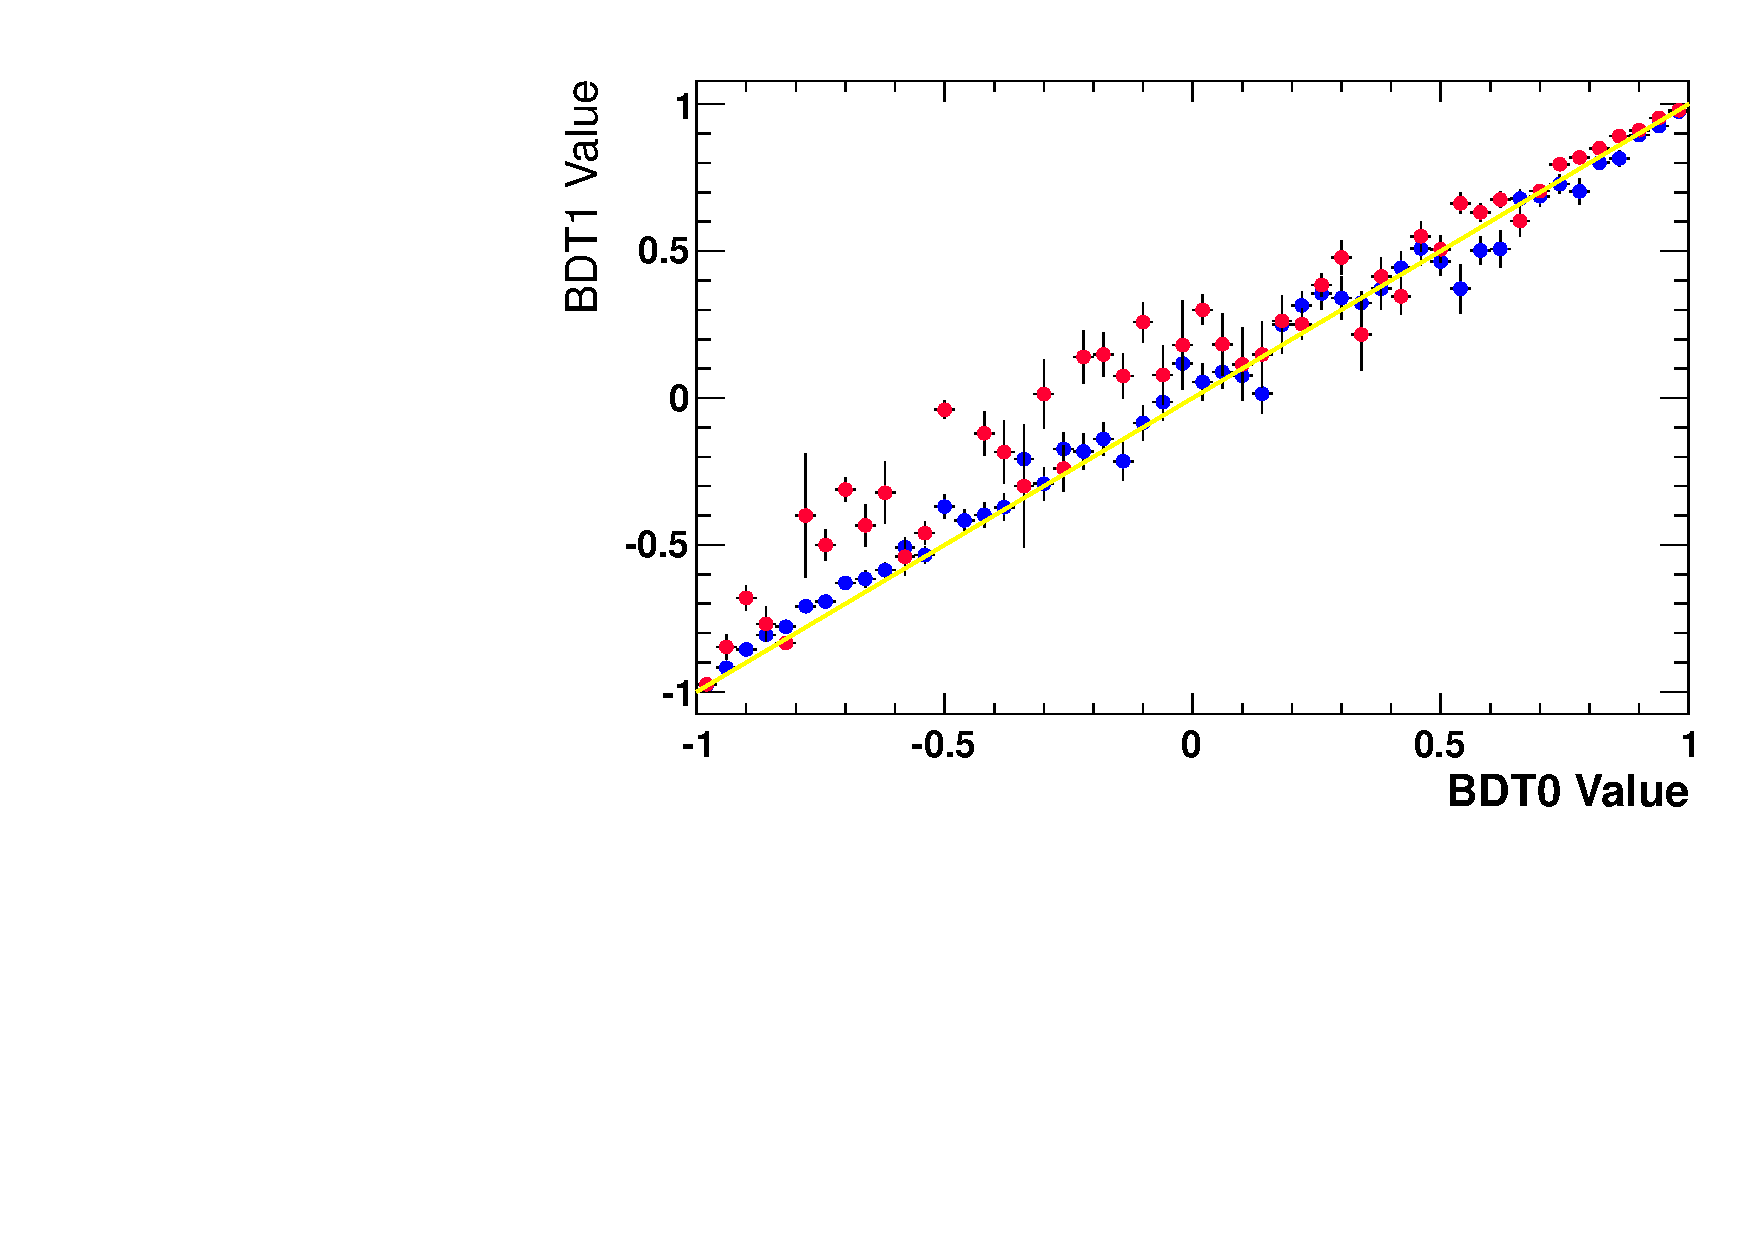
\includegraphics[width = 0.49 \textwidth]{mcBDT.pdf}}
\subfigure{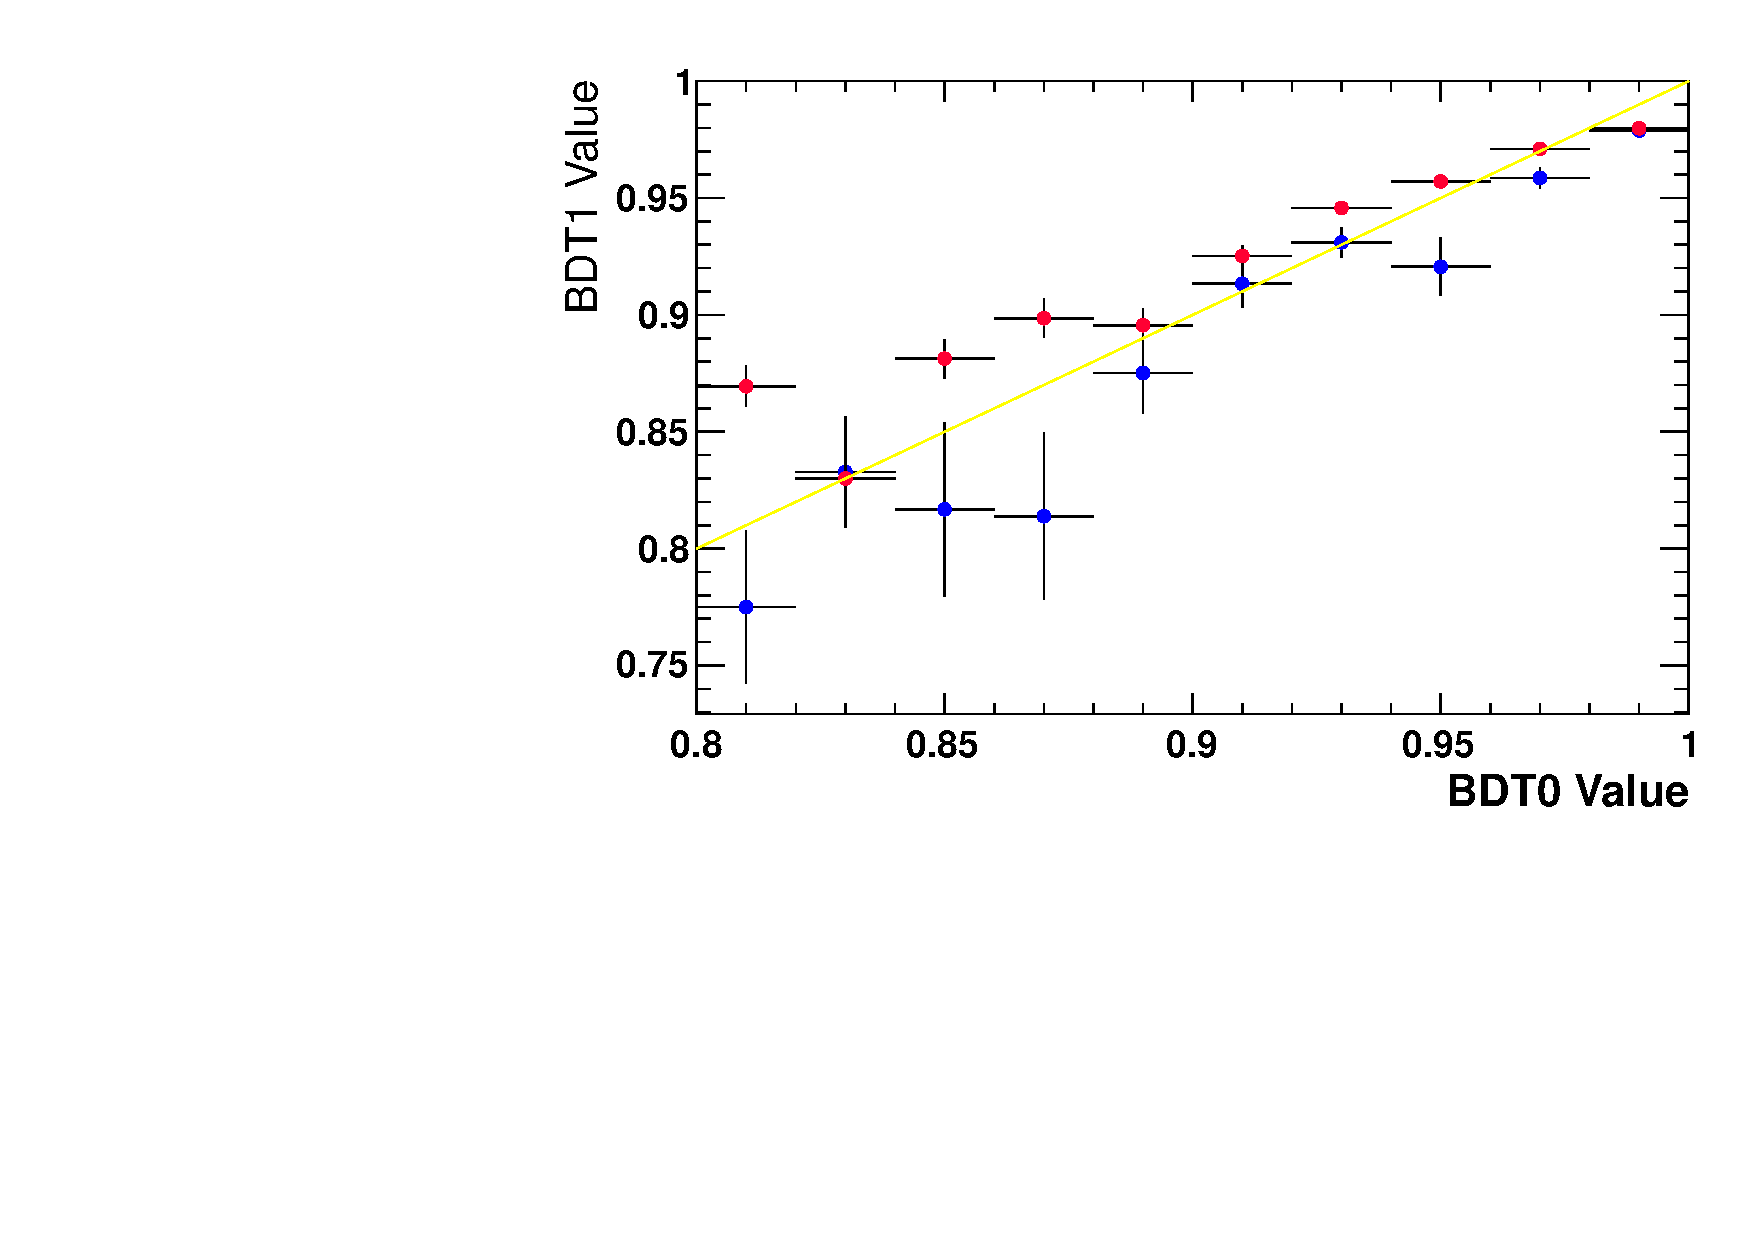
\includegraphics[width = 0.49 \textwidth]{mcBDT_ZOOM.pdf}}
\end{center}
\caption{\textit{\bdtn response on the \BdKstee Monte Carlo (red dots) and \lhcb data (blue dots). Each point represents the average value of \bdtb for a given bin of \bdta value. In the left plot a zoom on the region around the working point of the \bdtn cuts can be seen.}}
\label{fig:bdtvsbdt}
\end{figure}
\newpage

\section{Optimisation of the selection}
\label{sec:opti}
In order to guarantee the best selection of the \BdKstee candidates a 2-dimensional optimisation of the cut on the BDT and the \dllepi is performed. This optimisation is performed for the three trigger categories independently. As explained in Section \ref{sec:strategy} the \bdta is optimised on the data sample A2 and \bdtb is optimised on B2.\\
The optimal combination of cuts is found by maximising the variable $x = \frac{S}{\sqrt{S+B}}$, where $S$ stands for the number of signal events and $B$ the number of background events in the signal window. Therefore $S$ and $B$ are calculated for every cut combination. The cut on the \dllepi is varied between $>0$ and $>3$ in steps of 1. The cuts on \bdta and \bdtb are varied between $> \, 0.8$ and $> \, 0.98$ in steps of 0.2.\\

\subsection{Estimation of signal candidates $S$}
The number of signal events is calculated using a combination of Monte Carlo and \lhcb data for the \BdKstee and the \BdToJPsieeKst decays.
\begin{eqnarray}
S(\BdKstee) = S(\BdToJPsieeKst) \cdot  & \frac{\epsilon^{sel}(\BdKstee)}{\epsilon^{sel}(\BdToJPsieeKst)} \nonumber \\
 &\frac{\BR(\BdKstee)}{\BR(\BdToJPsieeKst)}
\end{eqnarray}
The ratio of selection efficiencies $\frac{\epsilon^{sel}(\BdKstee)}{\epsilon^{sel}(\BdToJPsieeKst)}$ are obtained from the Monte Carlo while the number of \BdToJPsieeKst signal events after the selection S(\BdToJPsieeKst) is computed from \lhcb data. The strategy of combining Monte Carlo and \lhcb data is chosen because the Monte Carlo does not reproduce certain properties of the data such as the trigger behaviour or the distribution of the particle identification value. The ratio of efficiencies for the \BdKstee and the \BdToJPsieeKst on the other hand should be free of these systematic errors.\\
For the purpose of extracting $S(\BdToJPsieeKst)$ the same selection as for the \BdKstee candidates is applied with the exception $2400 \mevcc \, < \, m(\jpsi) \, < \, 3400 \mevcc $ instead of the $m(\epem) $ cut. \\
As in the reweighting procedure for $nPV $ the constrained on the \jpsi mass is applied. To extract $S(\BdToJPsieeKst)$ a function consisting of a double Crystal-Ball distribution \cite{crystal} representing the signal and a exponential representing the background is fitted to the \Bd mass.
An example can be seen in Figure \ref{fig:ex1} on the left.\\

\subsection{Estimation of background events $B$ in the signal window}
The background is estimated from the \BdKstee \lhcb data.
Therefore the signal region is blinded and an exponential function is fitted to the sidebands which describes the background distribution to a first approximation. For the fit result the amount of background events is extrapolated. An example of the fit to the background can be seen in Figure \ref{fig:ex2}.\\

\begin{figure}[ht]
\vspace*{-0.5cm}
\begin{center}
\subfigure{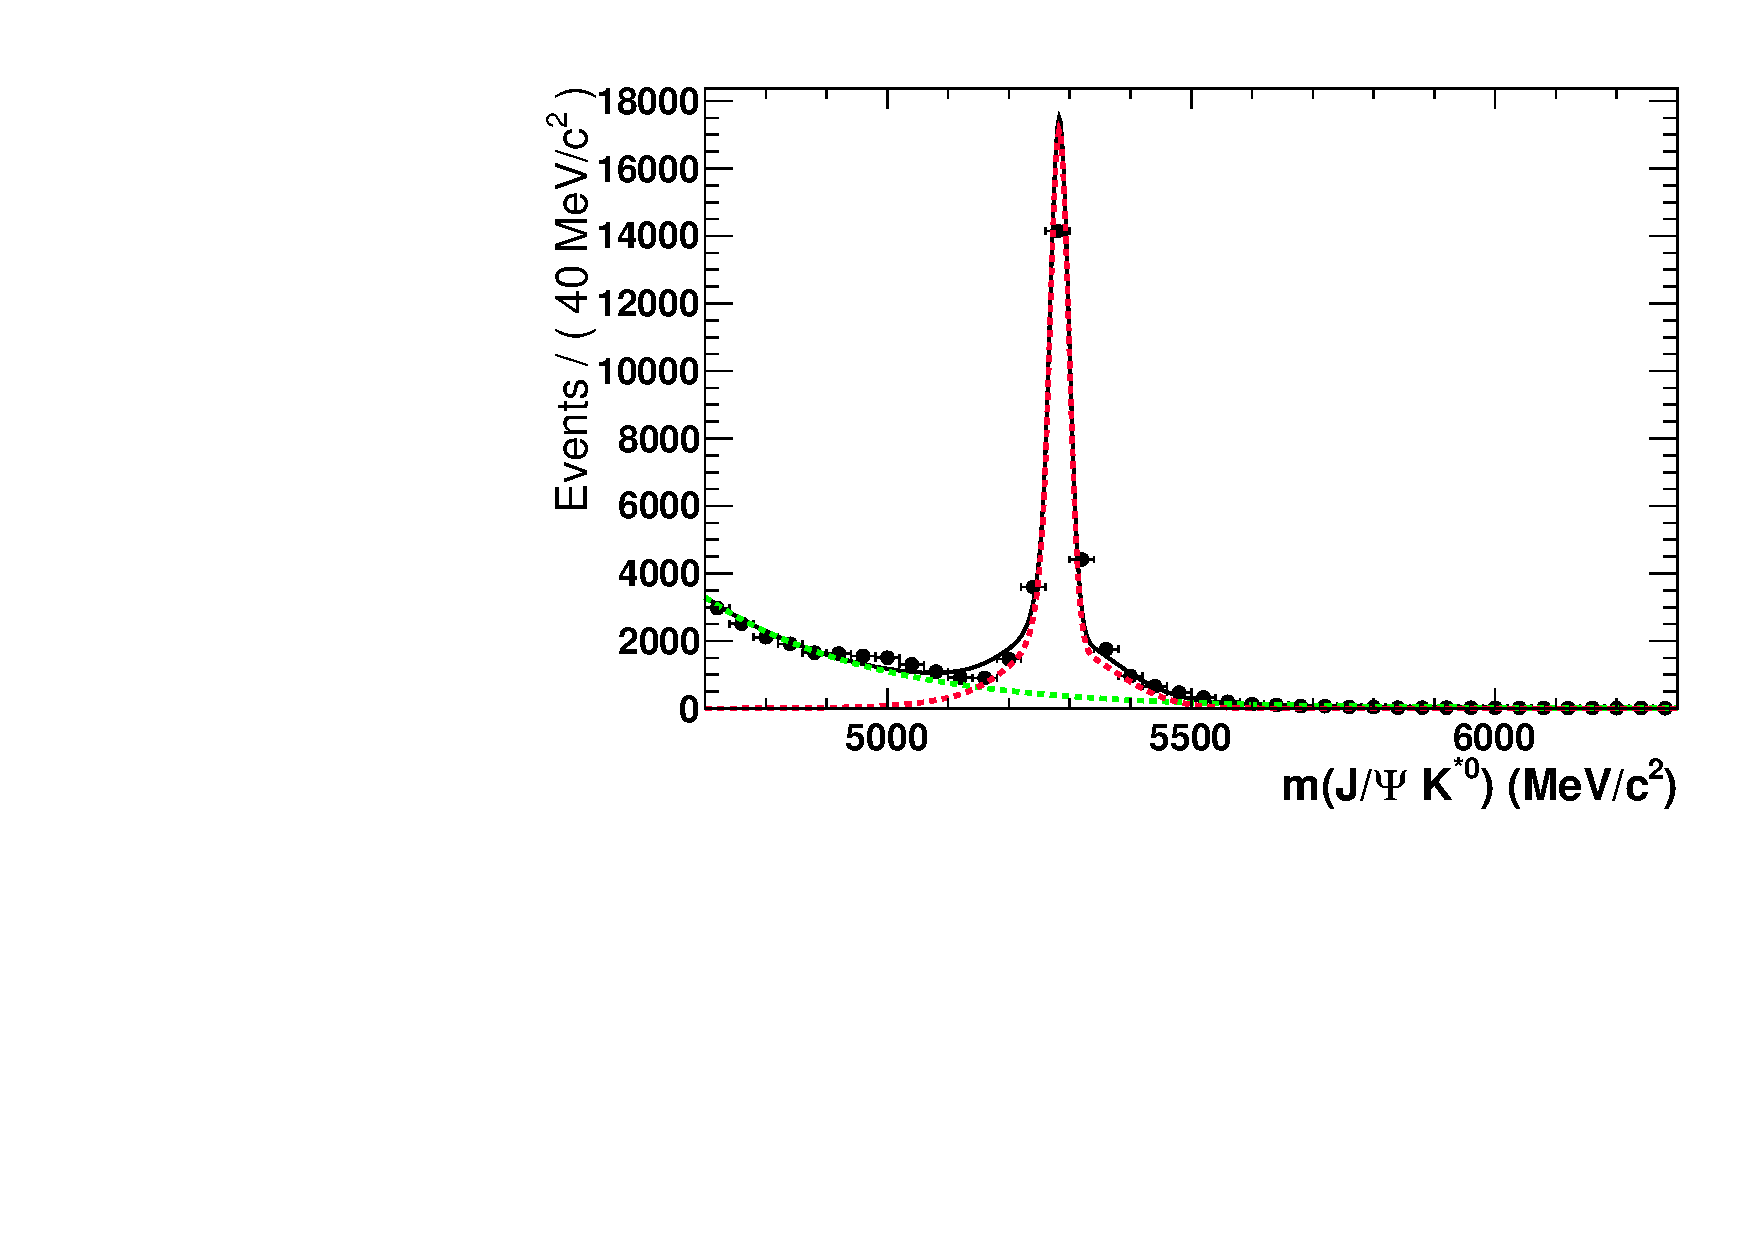
\includegraphics[width = 0.49 \textwidth]{BDT0_signalesti.pdf}\label{fig:ex1}}
\subfigure{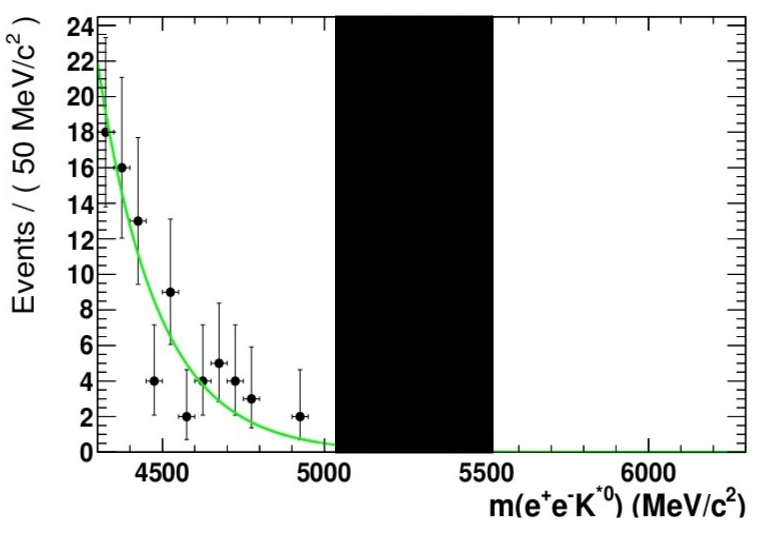
\includegraphics[width = 0.49 \textwidth]{bkgest.jpg}\label{fig:ex2}}
\end{center}
\caption{\textit{\textbf{Left}: Sample B2 \Bd mass distribution from the \BdToJPsieeKst with the cut combination \bdta > 0.88 and \dllepi > 1. Black points: \lhcb data, pink curve: signal \PDF, green curve: \PDF for the combinatorial background. \textbf{Right}: Sample B2 \Bd mass distribution from the \BdKstee with the signal window blinded with the cut combination \bdta > 0.88 and \dllepi > 1. Black points: \lhcb data, green curve: \PDF for the combinatorial background. }}
\label{fig:ex}
\end{figure}


\subsection{The optimised cut combination}
As has been shown in the previous section the values for the \bdta and \bdtb are in agreement for a given event. Therefore and for simplicity reasons the cut on the \bdtn value is chosen to be the same on \bdta and \bdtb within a trigger category. The optimisation is hence performed on one of the \bdtn values only. The Figures \ref{fig:optiele}, \ref{fig:optihad} and \ref{fig:optitis} show the value of $x = \frac{S}{\sqrt{S+B}}$ for the different combination of cuts on the \dllepi and the \bdtn value. The relative error on $x$ is between $5\, \%$ for the L0Electron category and $10\, \%$ for the categories with less statistics L0Hadron and L0TIS.\\
%It can be seen from these plots that the value of $x$ is already on a plateau meaning that the variation of $x$ over the displayed \dllepi and \bdtn value space. Furthermore \\


%\subsubsection{The \dllepi cut}
%The L0Electron category which has the highest statistics clearly prefers the cut of $\dllepi >1$. This statement is also true for the L0TIS category. \\
%The L0Hadron category prefers tighter cuts. However, the distribution of $x$ is not the only and best classifier of the cut combination. Taking into account the values of $S$ and $B$ separately it can be seen, that the tight cut on \dllepi removes a lot of background but also reduces the expected signal events. From these observations the cut on \dllepi for the L0Hadron category was chosen to be $\dllepi >1$. This selection is predicted to have a ration of $\frac{S}{B} \approx 1$ while keeping the signal yield at a significant level.\\
%
%\subsubsection{The \bdtn cut}
%As can be seen in Figures \ref{fig:optiele} and \ref{fig:optitis} the L0Electron and the L0TIS category have both a preferred cut value of $\bdtn \, >\, 0.88$ and $\bdtn \, >\, 0.92$ respectively. Again, Figure \ref{fig:optihad} for the L0Hadron category does not give a clear indication of which \bdtn cut is optimal. However, taking into account the distributions of the signal yield $S$ and the estimated number of background $B$ the chosen cut of $\bdtn \, >\, 0.9$ was chosen.
\begin{figure}[ht]
\begin{center}
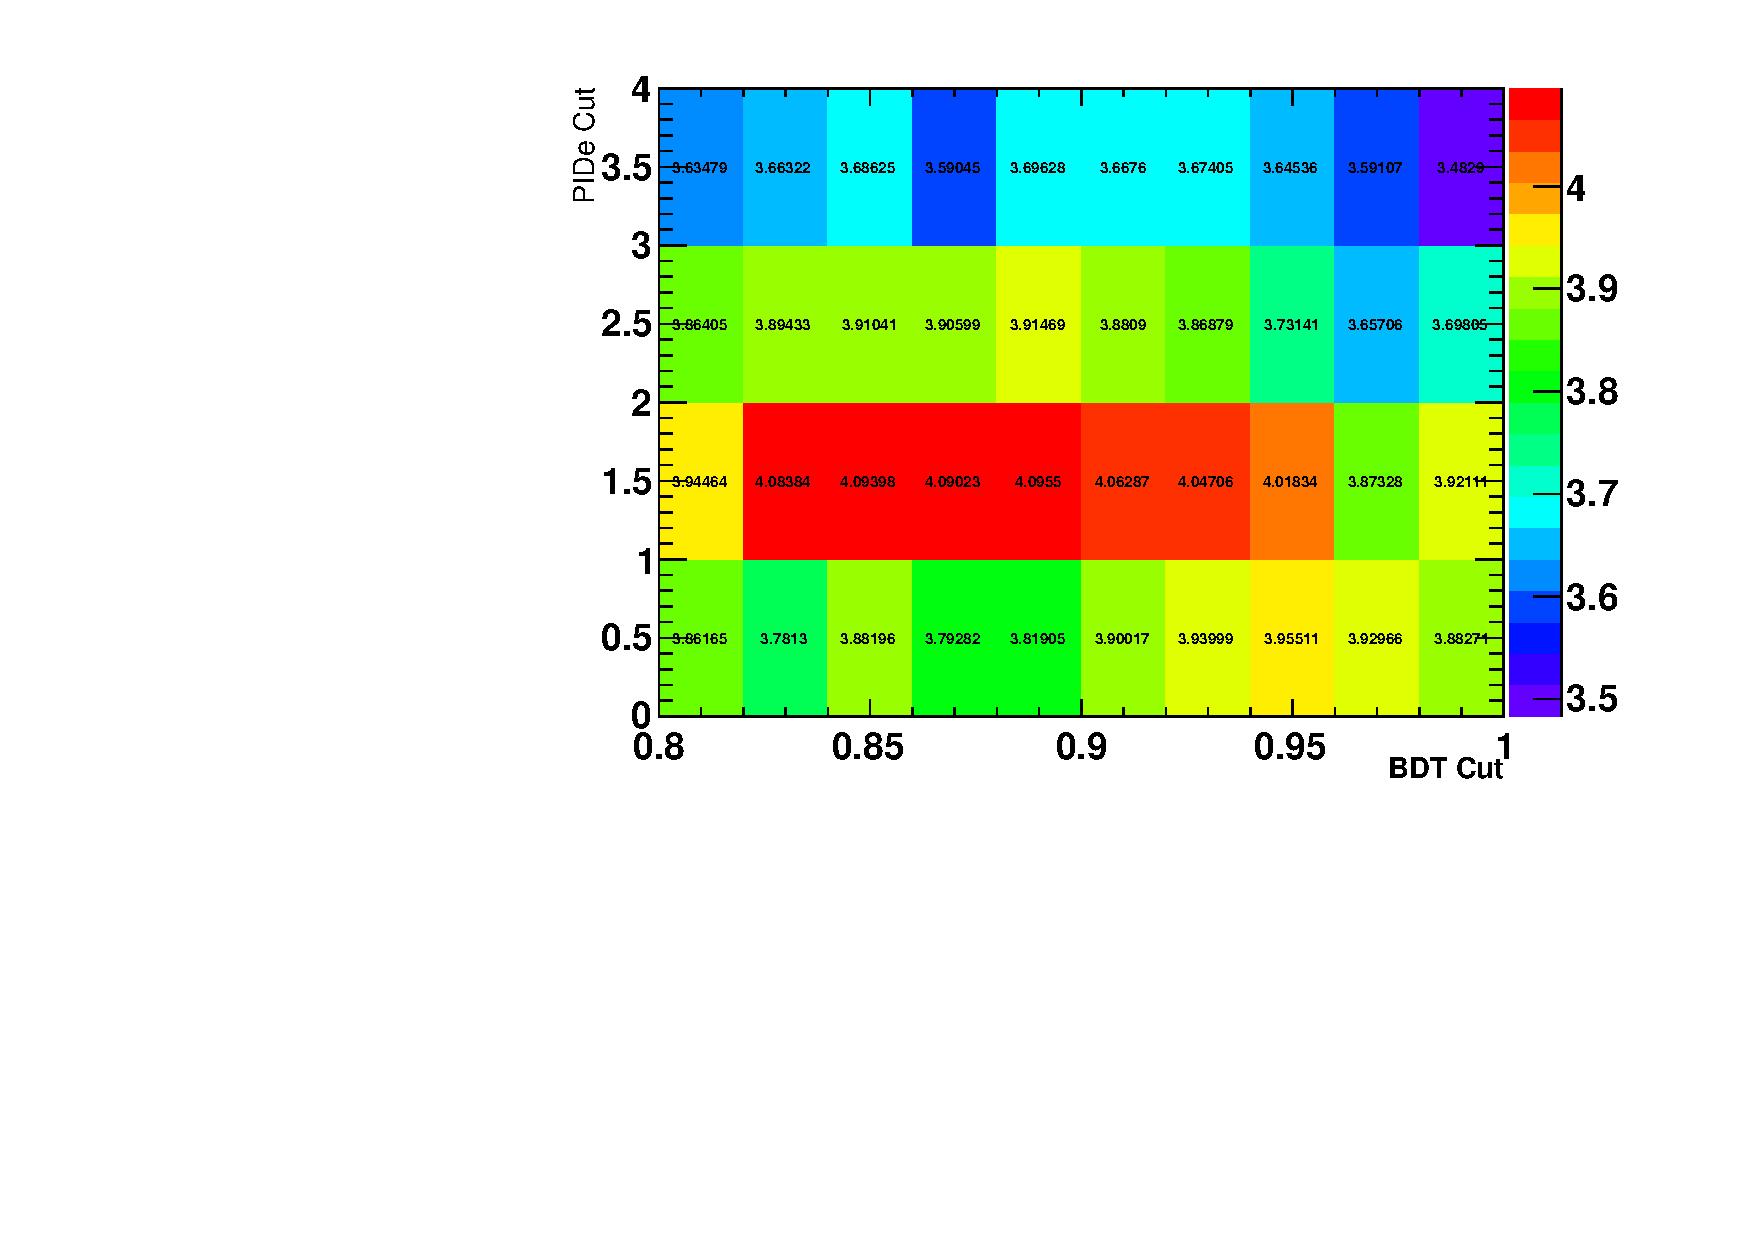
\includegraphics[width = 0.8 \textwidth]{BDT_L0Ele_opti.pdf}
\end{center}
\vspace*{-1cm}
\caption{\textit{The variable $x = \frac{S}{\sqrt{S+B}}$ for different combinations of the cut on \dllepi and the \bdtn value evaluated for the events in the L0Electron category. The error on $x$ is about $5\, \%$.}}
\label{fig:optiele}
\end{figure}

\begin{figure}[ht]
\begin{center}
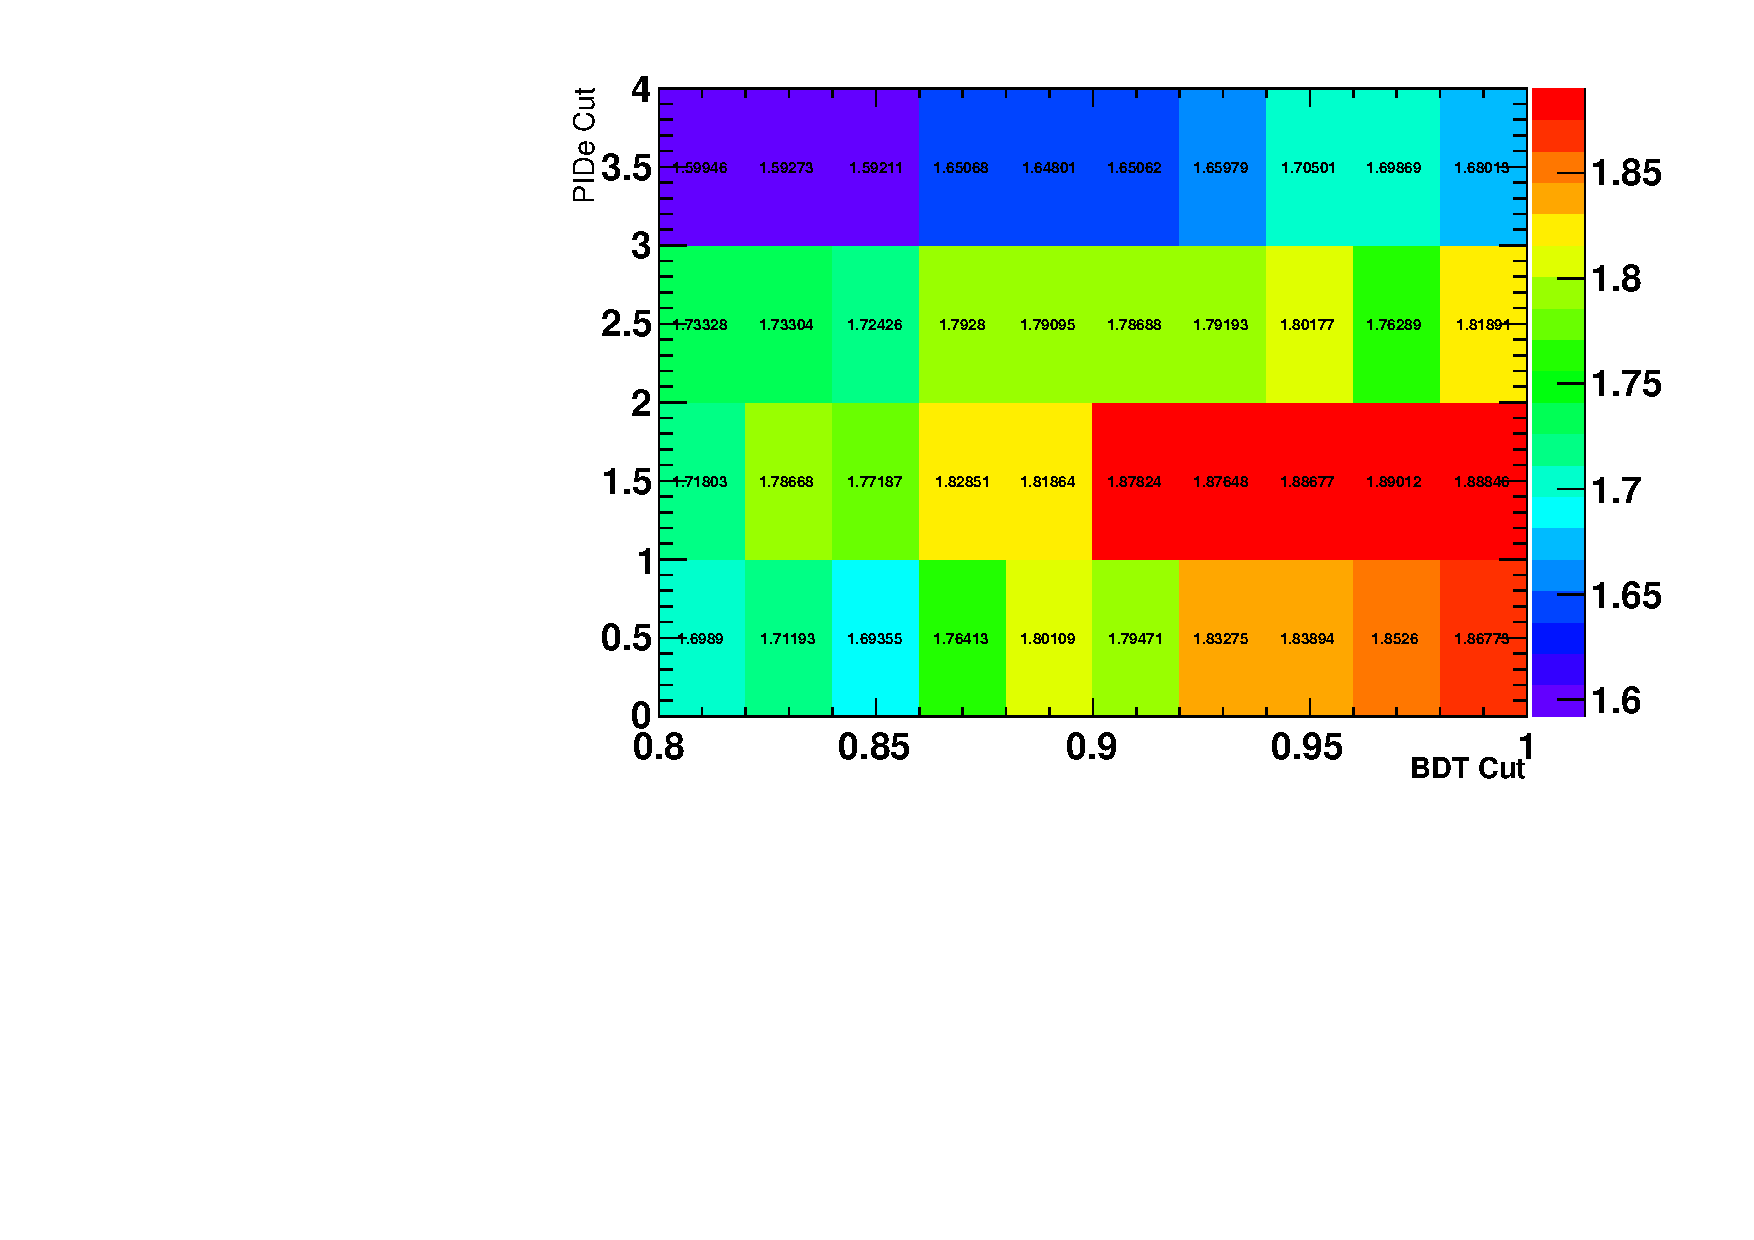
\includegraphics[width = 0.8 \textwidth]{BDT_L0Had_opti.pdf}
\end{center}
\vspace*{-1cm}
\caption{\textit{The variable $x = \frac{S}{\sqrt{S+B}}$ for different combinations of the cut on \dllepi and the \bdtn value evaluated for the events in the L0Hadron category. The error on $x$ is about $10\, \%$. }}
\label{fig:optihad}
\end{figure}
%\begin{figure}[ht]
%\begin{center}
%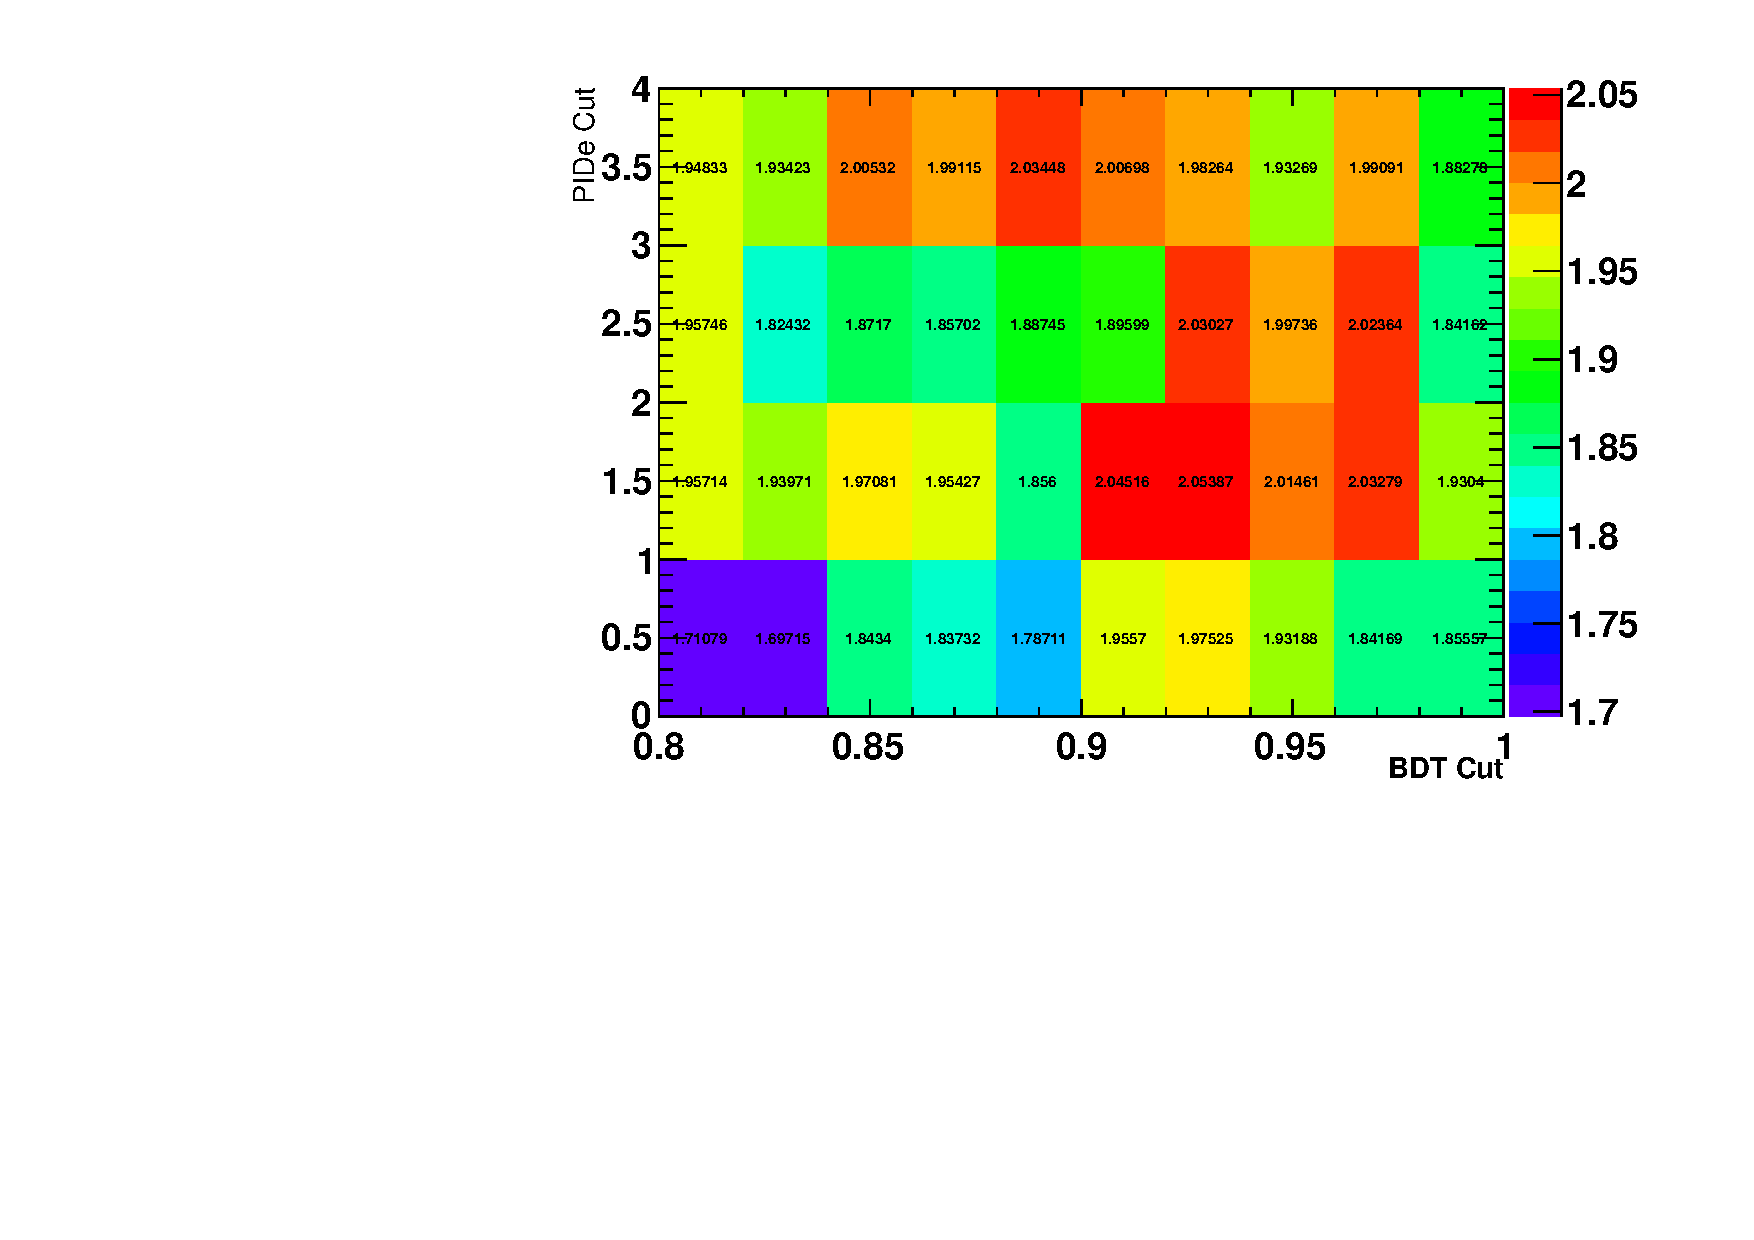
\includegraphics[width = 0.8 \textwidth]{BDT_L0TIS_opti.pdf}
%\end{center}
%\vspace*{-1cm}
%\caption{\textit{The variable $x = \frac{S}{\sqrt{S+B}}$ for different combinations of the cut on \dllepi and the \bdtn value evaluated for the events in the L0TIS category. The error on $x$ is about $10\, \%$. }}
%\label{fig:optitis}
%\end{figure}
\noindent%
\begin{minipage}{\linewidth}
\makebox[\linewidth]{%
  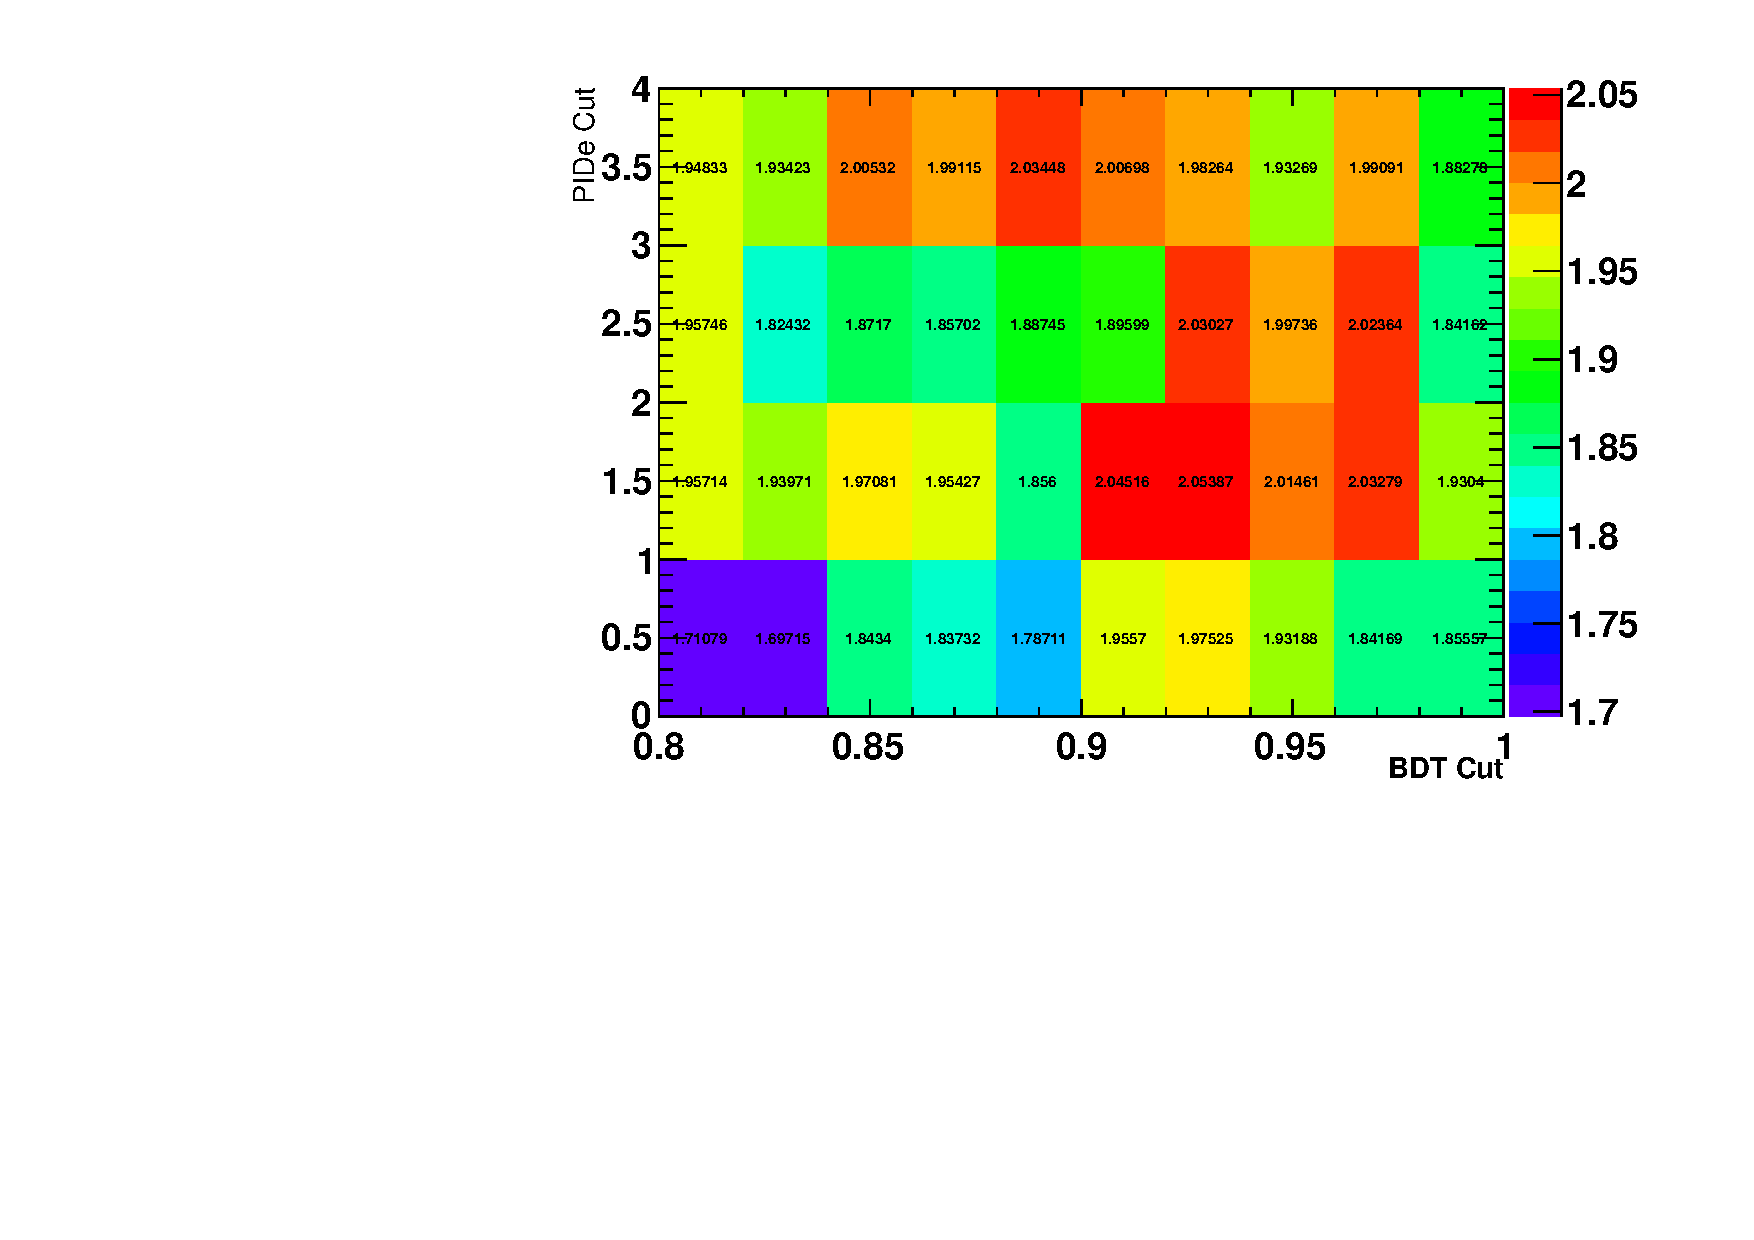
\includegraphics[width=0.8\textwidth]{BDT_L0TIS_opti.pdf}}
  \vspace*{-1cm}
\captionof{figure}{\textit{The variable $x = \frac{S}{\sqrt{S+B}}$ for different combinations of the cut on \dllepi and the \bdtn value evaluated for the events in the L0TIS category. The error on $x$ is about $10\, \%$. }}
  \label{fig:optitis}
\end{minipage}

From Figure \ref{fig:optiele}, \ref{fig:optihad} and \ref{fig:optitis} the working points can easily be determined since the distributions of $x$ have each a local maximum. This lies at $\dllepi >1$ for all three trigger categories and at $\bdtn \, >\, 0.88$, $\bdtn \, >\, 0.9$ and $\bdtn \, >\, 0.92$ for L0Electron, L0Hadron and L0TIS respectively.\\

\begin{table}[ht]
\begin{center}
\begin{tabular}{c|c|c}
 & \dllepi cut & \bdtn cut\\
 \hline
 \hline
 L0Electron & $\dllepi \, > \, 1$ & $\bdtn >0.88$\\
 \hline
 L0Hadron & $\dllepi \, > \, 1$ & $\bdtn >0.9$\\
 \hline
 L0TIS & $\dllepi \, > \, 1$ & $\bdtn >0.92$\\
\end{tabular}
\end{center}
\caption{\textit{Results of the optimisation of the cuts on \dllepi and the \bdtn value for the three independent trigger categories.}}
\label{tab:bdtcuts}
\vspace{1cm}
\end{table}


\section{Veto cuts against specific background contamination}
While the \bdts show very good performance in rejecting the combinatorial background other more specific sources of background are not gravely affected by the \bdtn cuts. One of this background sources is the $\Bd \rightarrow \Dm \ep \neu$ decay that was discussed in Section \ref{sec:denu}. This background is now suppressed by the cut $\ctl <0.8$.\\
However, there are two other specific backgrounds that contribute to the contamination of the \BdKstee candidates. They will be discussed in the following.\\

\subsection{The $\Phi \rightarrow \Kp \Km$ veto cut}
The decay $\Bs \rightarrow \Phi \epem$ is expected to have a branching ratio of the same order as the \BdKstee. Since the kinematics are similar and since
the $\Phi$ meson has a branching ratio of $50\, \%$ for decaying into two charged charged kaons it is important to reject this specific background. If one of the kaons is misidentified as a pion the $\Phi$ could be reconstructed as a \Kstarz. While this background is already suppressed by the cuts on the particle identification variables for the kaon and the pion there is still a visible contribution from the $\Phi \rightarrow \Kp \Km$. This background can be suppressed further by calculating the mass of the $m(\Kp \Km)$ by assigning the pion-track the mass of a kaon. The distribution of this $m(\Kp \Km)$ variable is shown in Figure \ref{fig:masskk}. \\
The cut against the contamination from the $\Phi \rightarrow \Kp \Km$ is suppressed by a cut of $m(\Kp \Km)>1040\mevcc$\footnote{$m(\Phi) = 1019 \mevcc$\cite{pdg}}.\newpage
\begin{figure}[ht]
\begin{center}
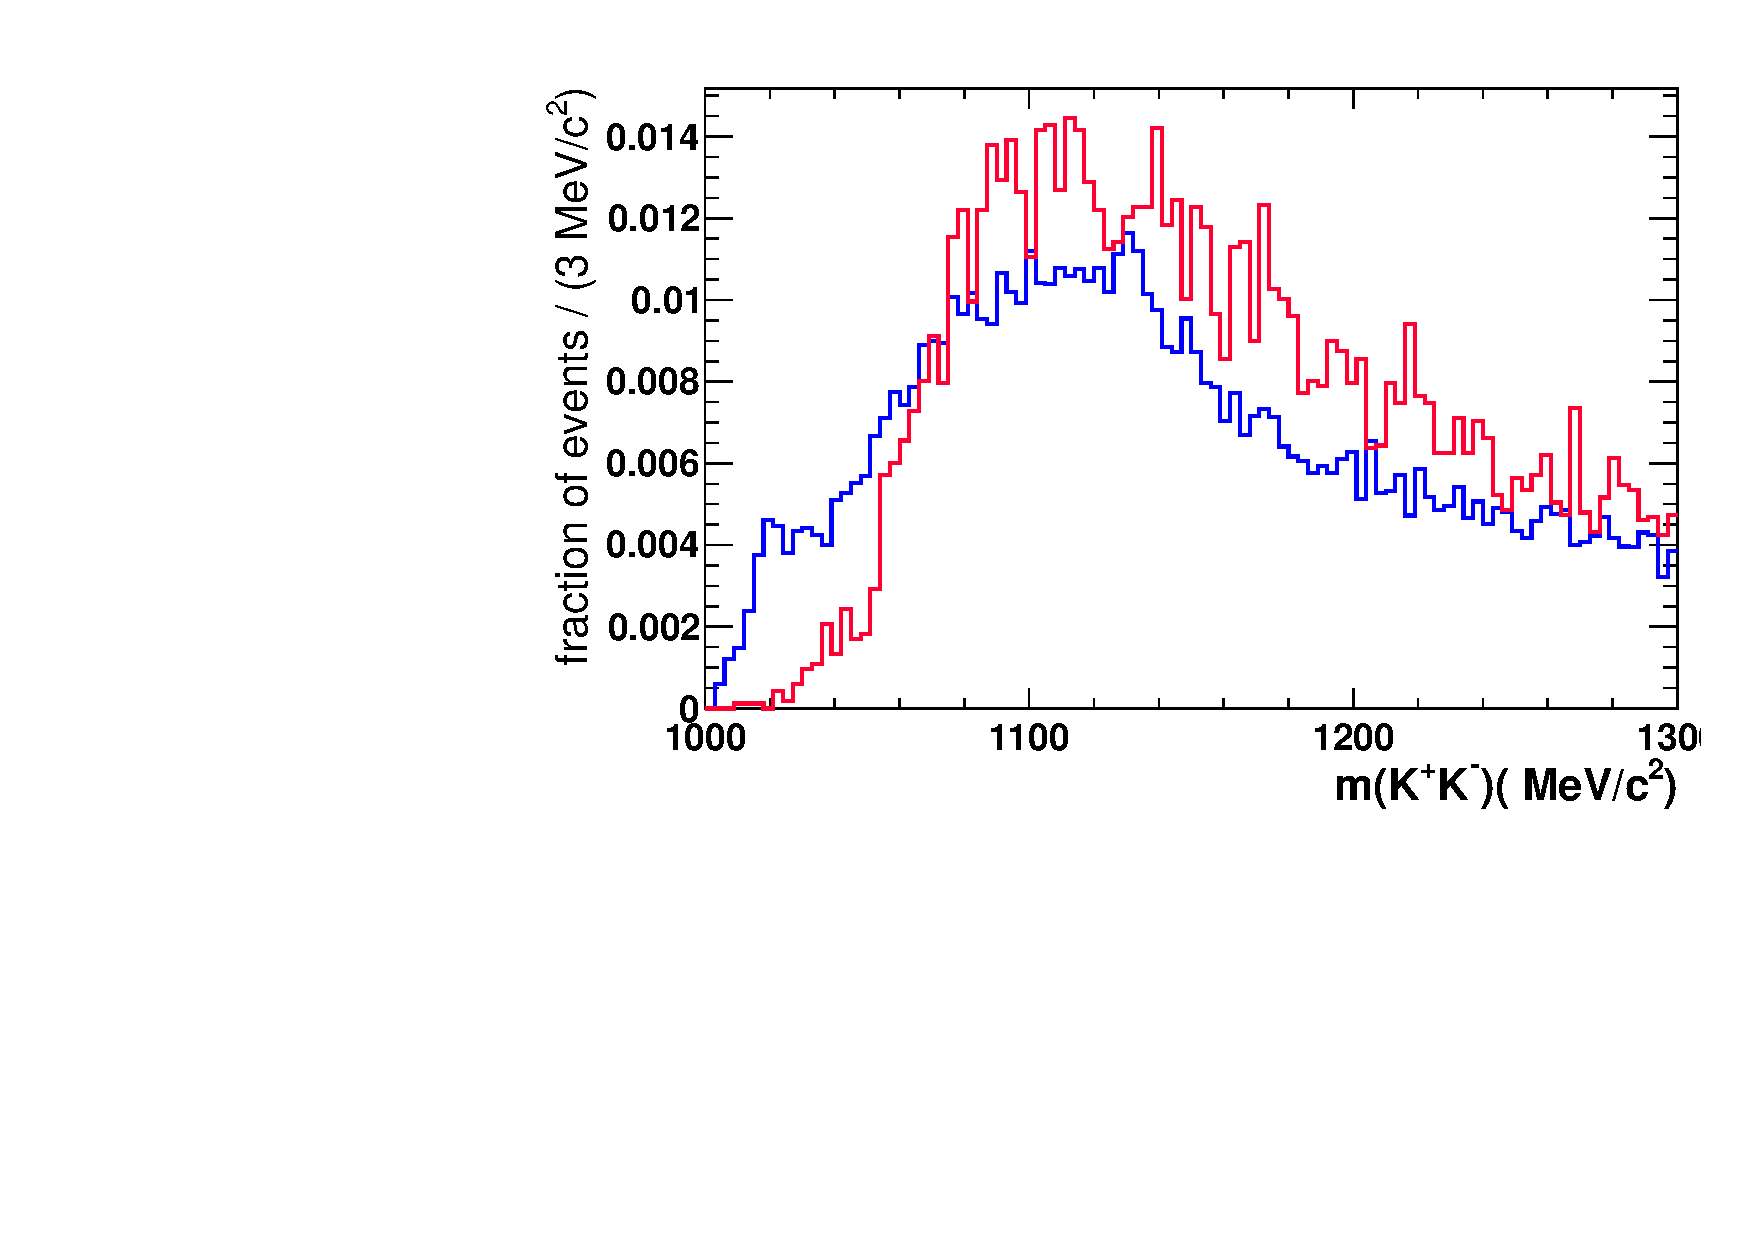
\includegraphics[width = 0.5\textwidth]{masskk.pdf}
\end{center}
\vspace*{-0.8cm}
\caption{\textit{Distribution of the $m(\Kp \Km)$ variable calculated under the assumption that the pion from \BdKstee is a misidentified kaon. The pink curve shows the distribution from the \BdKstee Monte Carlo while the blue curve is the distribution of the \lhcb data. Both samples were processed by the \BdKstee stripping20 line and underwent the preselection cuts. The data curve clearly shows a peak from the $\Phi \rightarrow \Kp \Km$ around 1020 \mevcc.}}
\label{fig:masskk}
\vspace*{1.5cm}
\end{figure}

\subsection{The \BdKstg veto cuts}
The \BdKstg decay has a branching ratio that is two orders of magnitude higher than the branching ratio of the \BdKstee decay and with the photon converting into two electrons the \BdKstg decay will look very similar to the \BdKstee decay. In \lhcb about $40\, \%$ of the photons convert before the calorimeter and while only about $10\, \%$ are reconstructed, the resulting \Bd mass peaks directly under the signal making it a particularly dangerous contamination.\\
Most of this background is removed by the lower cut on the $m(\epem) >20 \mevcc$. Additionally another cut has been developed to reject this background. Unlike for the \BdKstee decay, the $z$ coordinate of the \ep \en pair from the \BdKstg does not have to coincide with the \Kstarz vertex. If this coordinate is measured with a large error the \BdKstg may still be reconstructed as a \BdKstee decay. By applying a tight cut on the error of the $z$ coordinate $\sigma_z(\epem)$ this background can already be suppressed.\\
Even after this cut the \BdKstg decay can make a significant contribution to the \BdKstee signal peak. Therefore another cut is developed which takes into account that electrons from converted photons leave a different signature in the \velo stations (see Chapter \ref{chapter1}) than the electrons from the \BdKstee signal. In particular, the hits in the \velo for the electrons from converted photons commence at a larger $z$ coordinate than expected due to the flight distance of the photon before converting. Therefore a cut has been developed that takes into account the difference between the expected and the measured $z$ coordinate of the electrons first hit in the \velo. The expected $z$ coordinate of the electrons first hit in the \velo is calculated by extrapolating the position of the \Kstarz decay vertex in the direction of the electron momentum. The $z$ coordinate of the first \velo sensor that is crossed by this extrapolation is taken to be the first expected $z$ coordinate. This is illustrated in Figure \ref{fig:deltafm}.\\
A cut on this variable of $\Delta_z\, <\, 20 \mm$ has been found to be optimal. The cut on error of the $z$ coordinate of the (\epem) vertex was chosen to be $\sigma_z(\epem)<30\mm$. 
\begin{figure}[ht]
\begin{center}
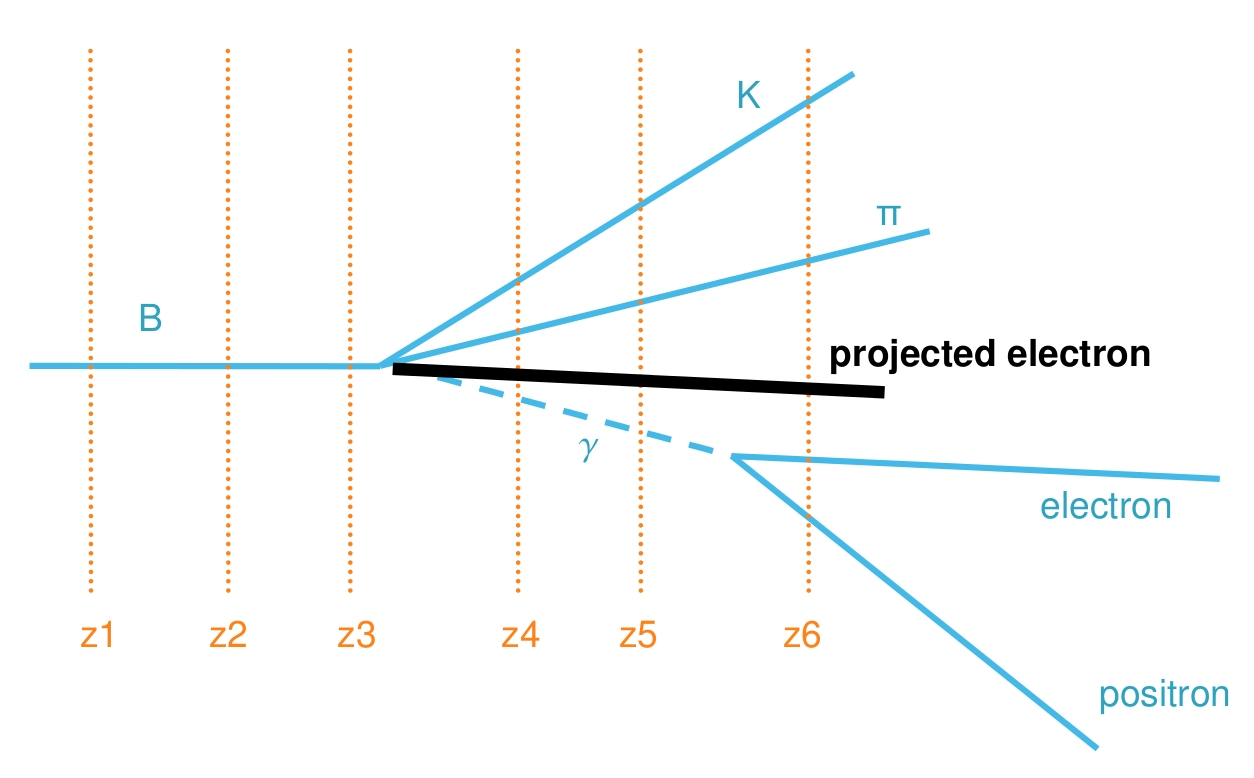
\includegraphics[width = 0.6\textwidth]{deltafm.jpg}
\end{center}
\caption{\textit{Illustration of the calculation of the expected $z$ coordinate in the \velo sensors for the first hit of the electron. The expected $z$ coordinate of the electrons first hit in the \velo is calculated by extrapolating the position of the \Kstarz decay vertex in the direction of the electron momentum. The $z$ coordinate of the first \velo sensor that is crossed by this extrapolation is taken to be the first expected $z$ coordinate.}}
\label{fig:deltafm}
\end{figure}
